% MEng project --- 40 pages limit
%
\documentclass[10pt, a4paper, pdflatex, leqno, twoside, openright]{report}

% Define margins
\usepackage[a4paper,inner=40mm,outer=15mm,top=15mm,bottom=25mm,pdftex]{geometry}

\usepackage[T1]{fontenc} % polsih

% Harvard citation
\usepackage[square]{natbib}
\usepackage{cite} % BiTeX

\usepackage{multirow}

\usepackage{graphicx}
\usepackage{caption}
\usepackage{subcaption}
\usepackage{url}
\usepackage{listings}
\usepackage{minted}
\definecolor{Bkgd}{rgb}{0.98,0.98,0.98}

\usepackage{datetime}
\newdateformat{monthyeardate}{%
  \monthname[\THEMONTH] \THEYEAR}

% New commands
\newcommand{\ts}{\textsuperscript}
\newcommand{\HRule}{\rule{\linewidth}{0.5mm}}

\newenvironment{dedication}
  {\clearpage               % we want a new page
   \thispagestyle{empty}    % no header and footer
   \vspace*{\stretch{1}}    % some space at the top 
   \itshape                 % the text is in italics
   % \raggedleft            % flush to the right margin
   \raggedright             % flush to the right margin
   \par\setlength{\leftskip}{0.3\textwidth}\noindent\ignorespaces
  }
  {\par                     % end the paragraph
   \vspace{\stretch{3}}     % space at bottom is three times that at the top
   \clearpage               % finish off the page
  }

\usepackage{lipsum}

\usepackage{amsmath}
\usepackage{scalerel}
\DeclareMathOperator*{\Bigcdot}{\scalerel*{\cdot}{\bigodot}}

\begin{document}

\begin{titlepage}
  \begin{center}

\includegraphics[width=0.5\textwidth]{gfx/UOB-logo.png}~\\[2.5cm]

\HRule \\[0.4cm]
{\huge \bfseries
  {\Huge Building activity recognition model:}\\[0.1cm]
  learning Prolog rules and extracting features from spatio-temporal data\\[0.4cm]
}
\HRule \\[1.5cm]

    \begin{minipage}{0.4\textwidth}
      \begin{flushleft} \large
\emph{Author:}\\
Kacper B. \textsc{\textbf{Sokol}}
      \end{flushleft}
    \end{minipage}
    \begin{minipage}{0.4\textwidth}
      \begin{flushright} \large
\emph{Supervisor:} \\
Prof.\ Peter \textsc{\textbf{Flach}}
      \end{flushright}
    \end{minipage}

\let\thefootnote\relax\footnote{\hspace*{-1.7em}Level M/7 $|$ COMSM0130---40cp Individual Project}

\vfill % Bottom of the page
{\large \today}
  \end{center}
\end{titlepage}

\newpage
\thispagestyle{empty}
\mbox{}

\newpage
\thispagestyle{empty}
\mbox{}

% Acknowledgement
\begin{center}\textbf{Declaration}\\[1em]\end{center}
This dissertation is submitted to the University of Bristol in accordance with the requirements of the degree of Master of Engineering in the Faculty of Engineering. It has not been submitted for any other degree or diploma of any examining body. Except where specifically acknowledged, it is all the work of the Author.\\[1.5cm]
Kacper B.\ Sokol, \monthyeardate\today

\newpage
\thispagestyle{empty}
\mbox{}

% Abstract
\begin{abstract}
\thispagestyle{empty}
This project researches \texttt{Prolog}'s \emph{Inductive Logic Programming} approach to learn parametrised rules describing \emph{Activities of Daily Life} based on data acquired form smart-houses: residences equipped with variety of sensors.\\

To this end, a highly customisable smart-house data generator is constructed and capabilities of \texttt{Aleph} inductive logic programming framework are assessed on various spatio-temporal datasets. Subsequently, an \emph{Activity Recognition Model} is constructed based on data collected from simulations and Washington State University CASAS smart-house installations. Both single and multiple occupiers models are considered.\\

To achieve the aforementioned goals, signal issues such as noise and incompleteness among others are addressed. Furthermore, a method for the raw data transformation into logical facts is proposed and evaluated. Difficulties such as real-valued sensor output and time representation in first-order logic are described.\\

The second objective of this work is to examine the structure of used spatio-temporal data with a view to discover and form new features. To this end, the dependencies between sensors are identified and assessed in order to construct more informative features. Hence by extending the dataset with new features performance of any classification algorithm can be significantly boosted.\\

Finally, this work opens up possibility of \emph{Narrative Analytics}: an extension of the Activity Recognition Model transforming generated rules into \emph{natural language}. The proposed data visualisation technique produces a plain English description of monitored residence, hence house situation can be examined without time consuming data interpretation.\\

The main utilisation of proposed here techniques is house monitoring for healthcare applications. SPHERE Project hosted at the University of Bristol addresses increasing healthcare costs and decreasing quality of life by designing tools and techniques allowing patients to live at home regardless of their medical conditions.\\
The activity recognition approach described here aims at improving the classification results and presenting smart-house data in a more transparent way. To the best of my knowledge, presented here methods are first of their kind and has not been yet described in any scientific publication.

\begin{center}
Keywords: \textbf{Inductive Logic Programming, Prolog, Activity Recognition, Data Generation, SPHERE}

% \let\thefootnote\relax\footnote{\noindent This publication including source code is available as \texttt{GIT} repository at: \url{https://github.com/So-Cool/cognition}.}
\end{center}
\end{abstract}



\newpage
\thispagestyle{empty}
\mbox{}
\begin{dedication}
``\ldots~On each landing, opposite the lift-shaft, the poster with the enormous face gazed from the wall. It was one of those pictures, which are so contrived that the eyes follow you about when you move. BIG BROTHER IS WATCHING YOU, the caption beneath it ran.~\ldots''\\[1cm]

``\ldots~The telescreen received and transmitted simultaneously. Any sound that Winston made, above the level of a very low whisper, would be picked up by it, moreover, so long as he remained within the field of vision which the metal plaque commanded, he could be seen as well as heard. There was of course no way of knowing whether you were being watched at any given moment. How often, or on what system, the Thought Police plugged in on any individual wire was guesswork. It was even conceivable that they watched everybody all the time. But at any rate they could plug in your wire whenever they wanted to. You had to live did live, from habit that became instinct in the assumption that every sound you made was overheard, and, except in darkness, every movement scrutinized.~\ldots''\\[2cm]

Nineteen Eighty-Four, George Orwell
\end{dedication}


\newpage
\thispagestyle{empty}
\mbox{}

\newpage
\cleardoublepage
\pagenumbering{gobble}
\tableofcontents
\cleardoublepage
\pagenumbering{arabic}

% \newpage
% \thispagestyle{empty}
% \mbox{}

%===============================================================================
%===============================================================================
%===============================================================================
%===============================================================================
%===============================================================================
\chapter{Introduction\label{ch:introduction}} %Background
\setcounter{page}{1}
% -------- plain English -> explain to someone
% Start with motivation - what is the problem and why it's interesting
% SPHERE somewhere here
% and application - what to do with it
% give solution
% then technique - why technique is best for solution - and more technical details
% --------
% What the project will produce -> contribution
% level of technical challenge
% how the output will be assessed - evaluation
% --------

  \section{The activity recognition problem}
    \subsection{Outline} %Problem outline
The main aim of the project is to build an \emph{activity recognition model} for a \emph{smart house} monitoring purposes.\\

By large, a smart house is a residence that is fitted with variety of sensors like: motion, door, appliance, water, item, etc.; as well as more sophisticated monitoring devices like cameras, and depth cameras. The first kind of sensors generate raw output usually of a form \texttt{sensorID on}/\texttt{sensorID off}, while the latter type outputs complex signal that needs to be pre-processed to be used as a classifier input. Due to these sensor characteristics my work mainly focuses on the first type of sensors.\\

The activity recognition model adjusted for the presented above scenario is a set of techniques that applied to a real time signals generated by a smart house predict currently held activity. In a single resident case the prediction target is only an activity like \emph{cooking} or \emph{sleeping}; when the house is occupied by multiple residents a \emph{person} performing the task is also outputted. The best solution to the outlined problem should work in \emph{signal streaming environment} therefore producing real-time activity predictions with high precision.

    \subsection{Motivation\label{sec:applications}} %Problem motivation/Applications
% Why interesting -> it generalises to any spatio-temporal data therefore can be used
The activity recognition model is a special case of a \emph{predictive model} for \emph{spatio-temporal} data. In general, such techniques predict quantity of interest based on input data, which encode both location and time of the event of interest. Smart-house signals are considered spatio-temporal as each sensor is associated with fixed location and the changes of sensor state are logged with date-time information.\\
% Why is it needed -> spatio-temporal data is everywhere,
This generalisation has a wide variety of real-life applications therefore addressing problems defined as ``hard'' in the activity recognition literature would make a valuable contribution to the field. 
The first and foremost area of application is healthcare.
% Population ageing - society geting older,  SPHERE project

      \subsubsection{Healthcare: The SPHERE Project}
Allowing elderly people and clinical patients to live at home regardless of the health conditions they suffer can greatly benefit such individuals. In general, dwelling in a cosy environment causes less stress. Moreover, the individuals living at home free space at specialistic day care centres and hospitals.\\
Therefore, being able to monitor behaviour of the patients staying in their own houses and effectively describe their activities result in better health care. Such techniques facilitate quick response to any kind of incidents without disturbing monitored people unless necessary.\\

\begin{figure}
  \centering
  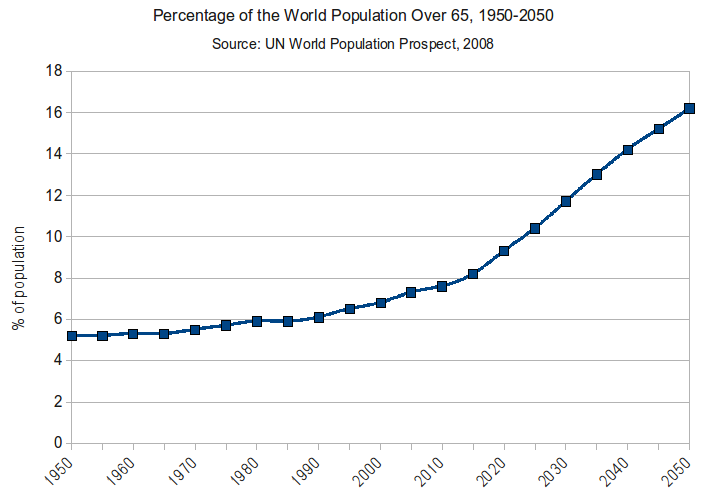
\includegraphics[scale=.5]{./gfx/populationOver65}
  \caption{Percentage of world population over 65, 1950--2050; \citep{populationAgeing}.\label{fig:agingPopulatiom}}
\end{figure}

% The Challenge
The problems of ageing population (see \emph{Figure~\ref{fig:agingPopulatiom}}), global population health issues, increasing healthcare costs, and decreasing quality of life are addressed by the \emph{SPHERE Project} hosted at the University of Bristol \citep{sphere}. This collaboration of clinicians, engineers, designers, social care professionals and various members of the public develops helpful technologies addressing real healthcare problems in a cost effective way.\\
The project focuses on developing real-world technologies which are acceptable in people's homes i.e.\ do not hinder their everyday-life. SPHERE works on both hardware and software smart house solutions: sensors and wearable devices as well as algorithms for healthcare applications. The first, are fitted into the place of interest to monitor it---generate various kind of signals, while the latter use the acquired information to identify any medical or well-being issues: predict falls, detect strokes, analyse eating behaviours, and detect periods of depression or anxiety.\\

My project extends the algorithmic part of undertaken by SPHERE research: I propose here novel data analysis framework to enrich suite of used activity recognition models.

      \subsubsection{Smart City}
The spatio-temporal data feeds are also common in variety of monitoring applications. One of them described by \citet{filipponi2010smart} is smart-city management. Automatic---quick and robust---analysis of traffic information, accident reports, etc.\ is invaluable in case of emergencies.\\
Among many possible applications, the data analysis can result in timely police intervention or well planned route for emergency services, therefore help in evacuation, crowd management, terrorist attack prevention and airport security control.

      \subsubsection{Complex Systems}
The spatio-temporal data are also produced in large quantities by many of complex system monitoring and control devices of: scientific facilities, buildings, data centres~\citep{moore2005data} and power plants~\citep{amin2005toward}. 
The tasks impossible to handle by humans either due to large data volume throughput or demand for low response time are vast area of application for the spatio-temporal data analysis. Such tools facilitate well suited to the needs system management and risk detection for tasks like: power distribution and balancing, nuclear reactor control, and data centre heat management to name a few.

      \subsubsection{Wildlife}
Monitoring animals behaviour in their natural habitat is an important source of information for many researchers~\citep{Szewczyk:2004:HMS:990680.990704}. Unfortunately, this task is very often impractical either due to an adverse climate or difficult access to the monitored place. Moreover, in many cases scientists want to avoid disturbing animals' life-cycle and habitats. Difficult access to such sites can be easily overcame with wide range of available sensors and analytic tools, majority of which share common ground with activity recognition task.

  \section{Contribution}
    \subsection{Existing work}
Over the last few years, building machine learning models for \emph{Activities of Daily Living} (ADL) has become an interest of many researchers. Its wide area of applications and increasing complexity appearing with every new discovery attracts now and then machine learning community with new and innovative solutions.

    \subsubsection{Techniques}
Up to date, extensive work on the smart houses occupied by \emph{single}~\citep{cook2009assessing,fatima2013unified} and \emph{multiple}~\citep{hsu2010strategies,singla2010recognizing,crandall2009coping} residents has been done. Vast majority of these studies focuses on the state-of-the-art learning algorithms such as:
\begin{itemize}
\item transfer learning---\citet{cook2013transfer},
\item conditional random field---\citet{hsu2010strategies,van2010activity},
\item support vector machines with various kernels---\citet{fatima2013unified},
\item hidden Markov model---\citet{rashidi2011discovering},
\item na\"{\i}ve Bayes---\citet{cook2013activity},
\item artificial neural networks---\citet{fatima2013unified,fatima2013analysis}.
\end{itemize}

All of these models are fuelled by variety of features extracted from the raw signals by a transformation and time manipulation. Majority of the undertaken work in this field uses the motion sensors as the main source for the feature construction with little to none attention to the item sensors.\\

Unfortunately, the scientific environment focuses on the mainstream techniques and forgets about less popular techniques that are possibly simpler and more suitable. Observing this gap in the spatio-temporal data analysis opens a vast new area of research: building the activity recognition models with uncommon these days machine learning techniques.

      \subsubsection{Datasets}
Training and testing any activity recognition model requires a dataset of recorded human activities. Such data can be only obtained by designing and building a testbed house fitted with variety of sensors followed by numerous activity recording sessions. As majority of the researchers cannot invest time or money to construct a smart house they use publicly available datasets generated by one of the research facilities. The most popular choice~\citep{fatima2013unified,fatima2013analysis,nazerfard2010conditional,cook2009assessing} among researchers are datasets published by \citet{cook2009assessing} working at the \emph{Center for Advanced Studies in Adaptive Systems}, Washington State University; also known as \emph{CASAS datasets}.\\
Their popularity is based on a variety of recorded activities---scripted and unscripted, with both single and multiple residents, available publicly free of charge. Furthermore, they are in general well formatted and documented nevertheless, they sometimes show labelling structure inconsistency.

      \subsubsection{Issues}
Tasks such as activity recognition aim at predicting a nearly infinite amount of human activities which can be performed in variety of manners. This enormous complexity of the task causes numerous problems with the activity prediction and the assignment of one of the multiple residents to the performed task. Such ``multi layered'' predictions yield many possibilities of performance assessment e.g.\ correct activity---incorrect resident prediction; correct activity---correct resident prediction; etc..\\

Moreover, the literature identifies building models for some of the activities as relatively difficult. Many of them involve complex, time consuming tasks with multiple residents crossing each others paths.\\

Finally, due to specific to a dataset output formatting and sensor name-space majority of learnt models are neither universal nor transferable.

      \subsubsection{Outcomes}
Unfortunately, outcomes of the activity modelling tasks reported in the literature are poor reference for assessing any model performance. Used datasets and fitness measures varies depending on the study making the result comparison impractical.\\
For instance,~\citet{fatima2013analysis} report \emph{accuracy} ranging from $\sim0.2$ to $\sim1.0$ depending on the model type, target activity and used dataset.

    \subsection{Project contribution}
Broad activity recognition literature and variety of tested therein models clearly indicate that no single classifier can handle the diversity of activity structures embedded in the data. Each model has its pros and cons therefore perfect solution should use all of the models each offering features not covered by the others---the concept known as an \emph{ensemble learning}.\\

Careful examination of the literature reveals missing discussion of the \emph{first-order} \emph{formulas}---parametrised logical rules, used as building blocks of the activity recognition model. My work comprehensibly covers this problem and expands collection of used techniques. Therefore, the main aim of the project is to apply an \emph{Inductive Logic Programming} (ILP) techniques to the spatio-temporal data acquired from ``smart'' installations---houses in particular---in order to build the \emph{Activity Recognition Model} and extract new, more informative features from the raw signals.\\

To address the first problem capabilities of an ILP system and possibilities of describing the model via a set of first-order logical rules are investigated. Both cases: the houses with a single and multiple occupiers are examined.\\
The latter task involves critical analysis of the smart house signals; activity specific feature design; and their quality assessment. Such novel signal characteristics can be then used in any other activity recognition model to boost its performance.\\

Designing a new activity model and signal features can become a difficult task when the exact structure of used dataset is unknown. Therefore, a systematic way of \emph{generating smart-house data} within user controlled environment is desirable. As part of this project a highly customisable data generator is proposed. Such a tool facilitates generating datasets representing activities of arbitrary complexity in the (in)deterministic world simulation, therefore a produced data can be used to build and test activity recognition models. Moreover, generated datasets are of invaluable help for systematic comparison of all the learning methods.\\

Finally, the project aims at proposing \emph{unified activity-recognition model evaluation measures}. A systematic way of assessing the performance of classifier in the activity recognition tasks is beneficial for comparing and contrasting multiple solutions. With such techniques an unambiguous assessment of multiple activity recognition methods is possible yielding straight forward identification of the best solution.

\section{Techniques}
To achieve outlined above goals the performance of proposed technique is evaluate on both \emph{CASAS datasets} and \emph{CASAS-inspired synthetic} datasets produced by the generator. Both datasets are translated from a log-like format into the \emph{knowledge representation} i.e.\ the sensor readings are expressed as logical facts. The classification result evaluation is made by the means of \emph{cross-validation}. CASAS datasets are split into separate trials to produce the folds; each containing all activities performed by a single experiment participant. On the other hand, when evaluating synthetic data each fold is generated independently with a common activity structure; small variation of order of used items; and multiple detours from originally planned motion trajectory.\\

% why I think it's best for the problem -> more details
The core of proposed technique is \texttt{Aleph}---Inductive Logic Programming system producing \texttt{Prolog} clauses as a data model. This approach to learning the activity recognition model was chosen as it lacks needed attention in the subject literature.\\
Proposed here rule based classifier greatly differs from currently used methods. Instead of employing \emph{propositional logic} it uses more powerful \emph{first-order logic} to express data and activity structure believes. More advanced ``grammar'' implies more possibilities to express the complex relations between the sensor events. This extra power can be harnessed to compose new data features, which in turn can be used in training other models and potentially improving their performance.\\

Furthermore, expressing the activity model in \texttt{Prolog} programming language brings to power all its advantages. Easy \emph{search space traversal} and built-in \emph{negation as failure} are invaluable tools in the feature construction process. Finally, learnt activity recognition model can be easily transformed to a \emph{generative model} for the data, hence serve as an activity example generator.\\
\texttt{Prolog} is also well known for its \emph{natural language processing} capabilities. A rule based model can be therefore used to produce \emph{Data Narrative}---a plain English interpretation of the data which supersedes any other visualisation technique targeted at the general public.\\

Another advantage of the ILP learning is use of a \emph{background knowledge}. It encodes \emph{clauses} needed to build the target model but can also contain any information or rules that might be beneficial for interacting with a raw data.\\
In the smart house model such component is of invaluable help as it can contain all the house and activity details that are absent in the raw data. Room layout, sensor placement, activity structure are just some of them.\\
Moreover, the background knowledge acts as a \emph{proxy} between the raw data and the model, making the latter universal. It means that in majority of cases the model learnt for one dataset can be applied to any other by using the data-specific background knowledge.\\

Very often the monitored activities exhibit hierarchy and structure. A rule based model allows to easily adjust the \emph{resolution of prediction}, therefore the activities can be described with a different level of depth. Considering the activity of eating, the model can simply predict the activity: \emph{eating}; it can also suggest the meal type (breakfast, lunch, brunch, etc.) based on the time of day; or even the food type (pasta, pizza, etc.) based on used ingredients.\\

A rule based model has one more distinctive feature not exhibited by many other machine learning models: it is \emph{human readable}. Such models are easy to inspect and tune simply by reading and modifying them. Moreover, the model rules can be easily evaluated whether they make sense. They can also help to discover any obscure information encoded in the data, hence gained knowledge can be used to design new, more suitable features in iterative manner. Rule manipulation is also feasible, therefore they can be simplified---by removing a predicate, extended---by appending a predicate, or combined---by enclosing them in a meta-rule.

\section{Deliverables}
% Deliverables / contribution -> what the project will result in
The project delivers a highly customizable smart-house data generator written in \texttt{Python}. It is publicly available as a \texttt{Git} repository\footnote{\noindent\url{https://github.com/So-Cool/SHgen}} to help researchers with training and testing the activity recognition models.\\
The smart-house simulator is highly customisable: room layout, motion and item sensor placement, and number of occupiers can be specified. The user designs an \emph{action script} which is then ``reconstructed'' by the house occupiers, what in turn produces sensor activations which are recorded in CASAS-like format.\\
As all the actions are ``directed'' a precise \emph{ground truth} information is available. Presence of the \emph{activity labels} in the data and precise control over the sensor interactions is of invaluable help in experiments of this kind. Finally, the data generator is proved to produces real-like data, therefore it is sound for use in the model creation and evaluation.\\
The generator repository contains detailed design and usage description to be easy to set-up and use for anybody. The choice of programming language was made based on its popularity making contribution, maintenance and development easy for the whole community.\\

Moreover, the project studies in great detail application of the ILP to various smart house settings. The knowledge representation of the house signals is proposed. Activity recognition problems defined in the literature as ``hard'' for both single and multiple residents are attempted and quality of results is discussed. The capabilities, limitations and advantages of the ILP in described scenario is thoroughly investigated and illustrated with examples. The role of the background knowledge encoding additional signal characteristics is examined. Used signal features are described and their role in the model construction is critically evaluated. Finally, the result evaluation techniques are proposed and used to score achieved results.

\section{Challenges}
Issues in all the layers: data, ILP and result evaluation arise. To overcome them, multiple solutions are presented and tested to select the best possible one for the smart house data analysis.\\

% prediction continuity issues, and readings in time continuity issues
Very often the data collected from smart-houses are corrupted or obscure due to incompleteness and sensor noise. This phenomenon leads to confusing gaps between ``observed'' actions causing model learning difficulties and intermittent prediction space. With help of the inductive learning such implicit information---describing intermediate steps between actions---can be inferred to overcome the rule creation difficulty and produce logically consistent scenario.\\
Moreover, the output of smart house installations is an unlabelled dataset. Filling the missing activity description is a manual labour, hence it is time consuming and prone to errors. Lack of the reliable ground truth information very often causes model learning difficulties.\\

Representing data in first-order logic has many advantages but it causes problems with unbounded variables like real numbers. This drawback imposes limitations on a time and real-valued sensor output representation which is crucial for a spatio-temporal data. Discovering possible representations and evaluating their usefulness is of great importance.\\

Learning a data model with the ILP is a complex process with number of intermediate steps. First, the learning environment of \texttt{Aleph} framework has to be configured to build the activity recognition model. For this purpose possible formats of the activity rule have to be discovered. Then, datasets and activity scripts need to be analysed to find any structures that can be used as the signal features. To this end, mechanism in a form of \texttt{Prolog} rules extracting quantities of interest form the raw data has to be built.\\
Background knowledge---the main component of \texttt{Aleph}---is a powerful tool. To make the best use of it, its capabilities and limitations must be discovered. To this end, usefulness of information not contained in the original dataset like room and sensor layout has to be assessed. Well designed background knowledge can significantly improve quality of used signal features.\\

Adjusting the resolution (level of detail) of achieved prediction is also an important task. Therefore, right balance in prediction detail and accuracy trade-off has to be found.\\
Handling data of a house occupied by multiple residents introduces difficulty of distinguishing them. Well known problem of agents sharing common space or crossing each other paths has to be resolved.\\

Finally, designing the most suitable an universal evaluation technique is crucial for results comparison. The main difficulty of this task are multiple classification error possibilities. The significance of each of them has to be considered to build performance metric that express real-life usefulness of proposed methodology.

\section{Result evaluation}
For the proposed generator to be publicly accepted in the community dealing with smart house activity recognition the proof of producing real-like data is necessary. Presented here proof is based on comparison of the activity models learn on the real and synthetic data and aims at assessing their similarities.\\

% OUtput asses ->
To prove importance of presented here activity recognition work a systematic and versatile evaluation technique is necessary. Firstly, a similar technique to the generator evaluation is used: comparison of models learnt on synthetic and genuine data. Moreover, the results of the rule based classifiers are compared against ``default accuracy'' i.e.\ accuracy achieved by \emph{majority class classification}.\\
Evaluation measures such as accuracy, precision, recall and F-measure are used. Overall, per activity, per person per activity statistics are presented. Furthermore, for single occupier cases the raw signals are translated into \texttt{ARFF} format and different machine learning models from \texttt{Weka} package are applied to them.\\
Finally, almost all presented here evaluation is based on \emph{cross validation} to make it more robust. The genuine data is split per trial so that each fold contains 5 different activities. The synthetic data is generated with random bits based on script corresponding to the genuine data.


%===============================================================================
%===============================================================================
%===============================================================================
%===============================================================================
%===============================================================================
\chapter{Spatio-temporal data\label{ch:stData}}
Spatio-temporal datasets are made of entries encoding events associated with location and their occurrence times. Such data are generated by monitoring systems, logging utilities and all kind of smart installations like houses and cities. Majority of such datasets are streamed, therefore it is implicitly assumed that learning algorithm at any point can look into the past but never see the future.\\
This assumption can be utilised in learning algorithms by allowing current prediction to be based on past predictions. Such practice is widely used to boost classifier performance, nevertheless it bears danger of skewing future predictions by propagating early made error.

  \section{The smart-house data}
My work focuses on smart house outputs, which are the most popular type of a spatio-temporal data. Each entry in such dataset is generated by change of sensor state and is characterised with \emph{time stamp}, \emph{sensor ID} (sensors are fixed at particular house location) and new \emph{sensor state}.\\
The smart house data owe their popularity mainly due to importance of the activity recognition models (see \emph{Section~\ref{sec:applications}}). Moreover, such datasets can be arbitrarily complex as there exist infinite amount of activities that they can represent. Therefore, techniques designed for the smart house data can be generalised for other spatio-temporal cases, which usually exhibit less complexity.

    \subsection{CASAS dataset\label{sec:csasDataDet}}
Washington State University's CASAS project~\citep{cook2009assessing} is the main source of real smart house datasets used in this study. These datasets are very popular in the activity recognition literature due to their large quantity, recorded in variety of testbeds with diverse sensor types: electricity, motion, door, item and appliance (fixed-phone, water, hob). Furthermore, they contain vast amount of activities of different complexity performed by single and multiple residents.\\
The datasets' structure is transparent; it is a list of sensor readings, one entry per line of the form:
$$
\text{\texttt{Date}~~\texttt{Time}~~\texttt{SensorID}~~\texttt{SensorState}~~(\texttt{PersonID\_ActivityID}~~\texttt{ActivityState}).}
$$
The first four columns are compulsory. The 5\ts{th} and 6\ts{th} sparse column contain the ground truth information and denote blocks of activities, which in multiple resident case are tagged with resident identifier. \texttt{ActivityID} is the name of activity like \emph{cooking}; \texttt{PersonID} is the resident identifier like \emph{residentA}; and \texttt{ActivityStatus} can be either \emph{begin} or \emph{end} where sensor activations placed between these the commands contribute to defined activity.\\
A snippet of CASAS dataset is shown in \emph{Figure~\ref{lst:CASASoneR}} for a single resident and in \emph{Figure~\ref{lst:CASAStwoR}} for two residents.

      \subsubsection{Single resident}
The two most popular CASAS datasets for single resident are \emph{\#1 WSU Smart Apartment ADL Normal Testbed} and \emph{\#2 WSU Smart Apartment ADL Error Testbed}, hence both are used in my project. The testbed---house and sensor layout---is shown in \emph{Figure~\ref{fig:house:oner}}.\\

\begin{figure}[htb]
  \centering%[width=.45\textwidth]
  \begin{subfigure}[b]{0.6\textwidth}
    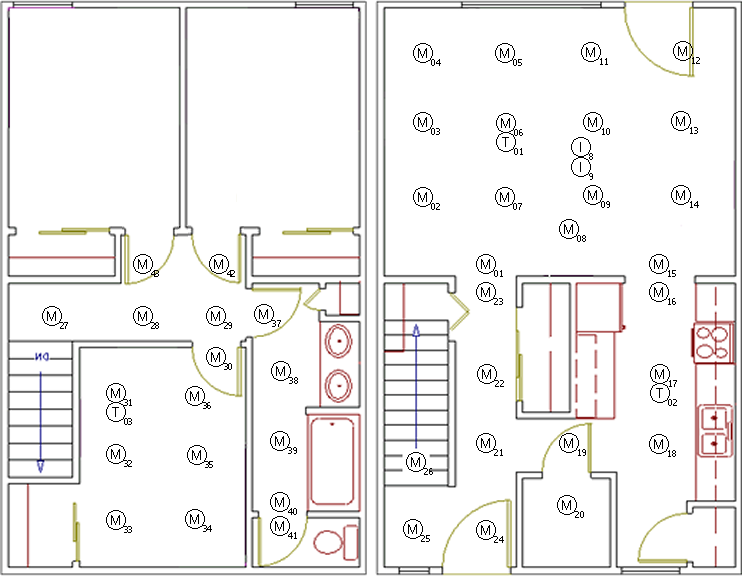
\includegraphics[height=6.3cm]{gfx/Chinook_3_Bedroom_TH}
    \caption{Apartment.\label{fig:house:oner:a}}
  \end{subfigure}%
  \begin{subfigure}[b]{0.3\textwidth}
    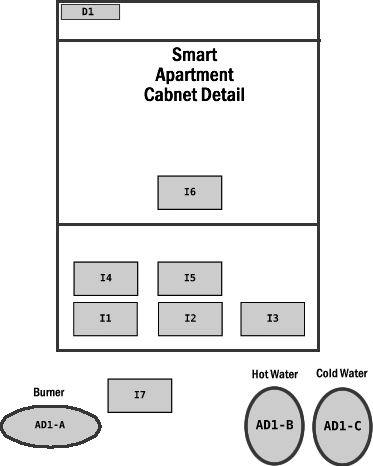
\includegraphics[height=6.3cm]{gfx/Chinook_Cabinet}
    \caption{Kitchen cabined.\label{fig:house:oner:b}}
  \end{subfigure}%
  \caption[The sensor layout of the testbed.]{Single resident testbed layout~\citep{cook2009assessing}.\label{fig:house:oner}}
\end{figure}

The following sensors fitted into the house living space were used in the experiment:
\begin{description}
\item[M$\Bigcdot\Bigcdot$] motion sensors; boolean signal: \emph{ON}, \emph{OFF};
\item[I$\Bigcdot\Bigcdot$] item sensors: oatmeal, raisin, brown sugar, bowl, measuring spoon, medicine container, phone book; boolean signal: \emph{PRESENT}, \emph{ABSENT};
\item[D01] cabinet door sensor; boolean signal: \emph{OPEN}, \emph{CLOSE};
\item[AD1-A, AD1-B] hot and cold water sensor; numerical, real-valued signal in range 0--1;
\item[AD1-C] burner sensor; numerical, real-valued signal in range 0--1;
\item[asterisk] phone usage; boolean signal: \emph{START}, \emph{END}.
\end{description}

The participants performed five scripted \emph{Activities of Daily Living}:
\begin{description}
\item[Make a phone call] Move to the phone in the living room; find a specific number in the phone book; dial the number; listen to the message; summarise cooking directions provided over the phone on a notepad.
\item[Wash hands] Move into the kitchen; wash hands in the sink with hand soap; dry hands with a paper towel.
\item[Cook] Cook a pot of oatmeal according to the directions given in the phone message: measure water, pour the water into a pot; boil the water; add oats; put the oatmeal into a bowl; add raisins and brown sugar.
\item[Eat] Take cooked oatmeal; take medicine container; move to the living room; eat the food.
\item[Clean] Take all of the dishes to the sink in the kitchen; clean them with water and dish soap.
\end{description}

The \emph{\#1 WSU Smart Apartment ADL Normal Testbed} dataset has the activity structure described above, while the \emph{\#2 WSU Smart Apartment ADL Error Testbed} has a systematic error introduced in each activity:
\begin{description}
\item[Make a phone call] Initially dial the wrong phone number, then redial;
\item[Wash hands] Leave the water on after washing hands;
\item[Cook] Leave the burner on after cooking the oatmeal;
\item[Eat] Forget to take the medicine container to the living room;
\item[Clean] Clean the dishes without water.
\end{description}

\emph{Figure~\ref{lst:CASASoneR}} shows example sensor readings which resulted from these tasks. They are annotated by hand with ground truth information.
\begin{figure}[htb]
\lstset{
  captionpos=b,
  frame=single,
  backgroundcolor=\color{Bkgd},
  rulecolor=\color{black},
  language=HTML,
  breaklines=true,
  % caption=CASAS single occupier dataset structure.,
  % label=lst:CASASoneR,
  float=tb
}
  \begin{lstlisting}
...
2008-02-26 10:52:58.577436 M17   OFF
2008-02-26 10:52:59.648222 M18   OFF       cook       begin
2008-02-26 10:52:59.792264 M17   ON
...
2008-02-26 10:53:43.512642 I02   ABSENT
2008-02-26 10:53:43.978491 I01   ABSENT
...
2008-02-26 10:53:52.112690 AD1-B 0.0421491
2008-02-26 10:53:54.721822 M17   ON        phone_call end
2008-02-26 10:53:55.107910 AD1-B 0.155979
...
  \end{lstlisting}
  \caption{CASAS single occupier dataset structure.\label{lst:CASASoneR}}
\end{figure}

      \subsubsection{Multiple residents}
The \emph{\#7 WSU Smart Apartment 2009 Two Resident Testbed} is the most popular choice among studies for multiple residents model training and testing. Its testbed design is presented in \emph{Figure~\ref{fig:house:twor}}, with the cabinet sensors layout same as in the single resident case---\emph{Figure~\ref{fig:house:oner:b}}.\\
\begin{figure}[htb]
  \centering%[width=.45\textwidth] % [height=6.3cm]
  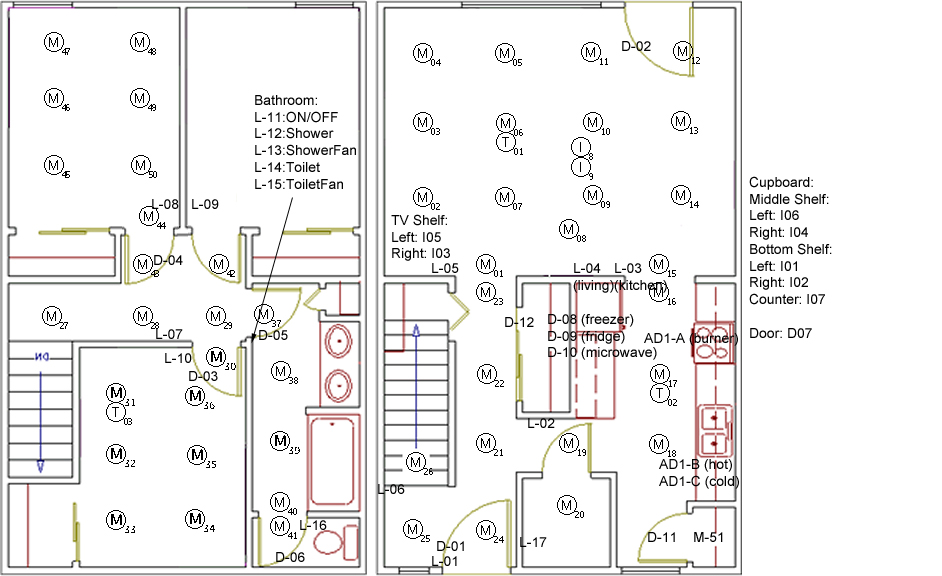
\includegraphics[height=6.3cm]{gfx/sensorlayoutTWOR.jpg}
  \caption[Two residents test-bed sensor layout.]{Two residents testbed layout~\citep{cook2009assessing}.\label{fig:house:twor}}
\end{figure}

In the multiple resident case the sensor set is extended with:
\begin{description}
\item[T$\Bigcdot\Bigcdot\Bigcdot$] temperature sensors; numerical, real-valued signal given in Celsius degrees; and
\item[P$\Bigcdot\Bigcdot\Bigcdot$] electricity usage meter; numerical, integer-valued signal given in kiloWatt hours.
\end{description}

This dataset was generated with two residents (\textbf{R$\Bigcdot$}): \textbf{R1} and \textbf{R2}, performing their \emph{normal daily activities} (not scripted), therefore their details are unknown:\\[1em]
\begin{tabular}{ l l l }
  \textbf{R$\Bigcdot$\_Bed\_to\_Toilet}, & \textbf{R$\Bigcdot$\_Personal\_Hygiene}, & \textbf{Wash\_Bathtub}, \\
  \textbf{R$\Bigcdot$\_Work}, & \textbf{R$\Bigcdot$\_Sleep}, & \textbf{Study}, \\
  \textbf{Meal\_Preparation}, & \textbf{Clean}, & \textbf{Watch\_TV}. \\
\end{tabular}
~\\[1em]

A snippet of CASAS multiple occupiers dataset is presented in \emph{Figure~\ref{lst:CASAStwoR}}.
\begin{figure}[htb]
\lstset{
  captionpos=b,
  frame=single,
  backgroundcolor=\color{Bkgd},
  rulecolor=\color{black},
  language=HTML,
  breaklines=true,
  % caption=CASAS two occupier dataset structure.,
  % label=lst:CASAStwoR,
  float=tb
}
  \begin{lstlisting}
...
2009-02-01 02:04:42.039332 P001 2812
2009-02-01 02:05:00.040187 P001 2797
2009-02-01 02:05:26.041714 P001 2784
...
2009-02-01 08:07:57.016506 T004 20.5
2009-02-01 08:07:57.826809 T002 21.5
2009-02-01 08:07:58.442939 T003 22
...
2009-02-06 11:28:36.666599 M09  OFF
2009-02-06 11:28:36.81007  M15  OFF  R2_prepare_lunch  end
...
2009-02-06 17:16:00.864039 M19  ON   Cleaning          begin
2009-02-06 17:16:01.061019 M21  OFF
...
  \end{lstlisting}
  \caption{CASAS two occupier dataset structure.\label{lst:CASAStwoR}}
\end{figure}

    \subsection{CASAS issues\label{sec:dataIssues}}
CASAS are the best smart house datasets that can be used for modelling activity recognition. Unfortunately, they exhibit issues common for every real dataset such as:
\begin{description}
\item[noise] random sensor activations;
\item[sensor failures] lack of sensor state change notification despite its proper usage; and
\item[incompleteness] signal discontinuity e.g.\ double sensor activation without deactivation in-between.
\end{description}
All of them cause difficulties in learning the activity recognition model.\\

Furthermore, CASAS specific drawbacks hinder their usage. Numeric output of the water and burner sensors is unexplained. Additionally, not all ground truth activity facts are assigned to people in the multiple residents datasets. Also, the activities in the multiple resident case are neither scripted nor explained in detail, therefore sensor output is tedious to analyse. Without good understanding of how the human actions affect the sensor activations it is relatively hard to design the activity recognition model.\\

All of these issues make testing an undocumented learning algorithm like the ILP difficult. Therefore, a highly customisable and precise smart house data generator is required.

  \section{The smart-house generator}
The smart house data generator created as a part of this project is intended to help in the activity recognition model design, training and testing. It is highly customisable, hence it gives the user great control over the generated data.\\

The user can design activities of arbitrary structure and complexity and use them to simulate the corresponding smart house output. Then, he can attempt to learn the structure encoded within it. As he knows the activity details, he can bypass real data issues (see \emph{Section~\ref{sec:dataIssues}}) and focus on tuning the model. Overcoming one issue at the time greatly benefits model quality and helps to identify its strong and weak points.\\

The tool is open source and published as a \texttt{Git} repository together with complete documentation describing design choices, usage details and input-output examples.

    \subsection{Capabilities}
To use the generator, firstly the user has to describe a house by stating room interconnections in a form of adjacency matrix.\\

Then, room layout and sensors placement within each room needs to be specified. The room dimensions are required together with a list of wanted sensors. The room design is based on Cartesian coordinates with origin in bottom left corner.\\
For motion sensors: ID, position and range has to be specified. Sensors of this type detect motion radially from their location.\\
Item sensors are defined with: ID, position, and its human readable name.\\
Finally, door location is needed for layout completeness. They are encoded with the \texttt{door} keyword, their coordinates and name of the room they lead to.\\
Example definition of each sensor type in preserved order is given in \emph{Figure~\ref{lst:sensorLayout}}.\\

\begin{figure}[htb]
\lstset{
  captionpos=b,
  frame=single,
  backgroundcolor=\color{Bkgd},
  rulecolor=\color{black},
  language=HTML,
  breaklines=true,
  % caption=Example sensor definitions.,
  % label=lst:sensorLayout,
  float=tb
}
  \begin{lstlisting}
living_room 6 6:
  m13  4.5 1   1
  i78  5.5 0.5 phone_book
  door 0   0.5 hall
  \end{lstlisting}
  \caption{Example sensor definitions.\label{lst:sensorLayout}}
\end{figure}

Subsequently, item sensors characteristic has to be specified. Each item, like TV, takes some time to use---average TV watching time. It is simulated by drawing a sample of Gaussian distribution with user specified mean and standard deviation. This feature is mainly used for simple activities, nevertheless the time can be altered in activity specification script (see the next paragraph).\\
Walking is simulated in a similar way---mean and standard deviation of a single step size and time have to be defined.\\

Finally, the activity script used to simulate interaction with the house sensors has to be provided. Arbitrary number of activities (they can be nested) for single or multiple residents can be defined. Each script begins with start position of the resident, which is followed by any of the atomic action commands: go to a room, go to a location within the room, use item (by simulating previously defined time), pick up an item or start a device, put down the item or turn off the device. For more complex activities any command can be used between starting/taking and stopping/returning any device/item.\\
Curly brackets together with an activity name are used to surround atomic actions contributing towards this activity. Example script is given in \emph{Figure~\ref{lst:path}}.\\

\begin{figure}[htb]
\lstset{
  captionpos=b,
  frame=single,
  backgroundcolor=\color{Bkgd},
  rulecolor=\color{black},
  language=HTML,
  breaklines=true,
  % caption=Example activity script.,
  % label=lst:path,
  float=tb
}
  \begin{lstlisting}
>ResidentA>
origin(hall)
go(kitchen)

cook{
  start(cabinet)
    do(oatmeal)
    do(pot)
  stop(cabinet)

  do(water_cold)

  start(burner)

  watchTV{
    go(living_room)
    do(tv)
  }watchTV

  go(kitchen)
  stop(burner)
}cook
<ResidentA<
  \end{lstlisting}
  \caption{Example activity script.\label{lst:path}}
\end{figure}

Presented here tool is capable of generating arbitrarily complex user defined activities by specifying their atomic actions. The generator can simulate single and multiple residents interacting with the house simultaneously.\\
Additionally to CASAS-like signals output, a precise ground truth information is recorded.\\

Datasets generated for the basic ILP activity recognition models are using testbed presented in \emph{Figure~\ref{fig:simHouse}} fitted with a systematic grid of motion sensors within each room.

\begin{figure}[htb]
  \centering% [width=.9\textwidth]
  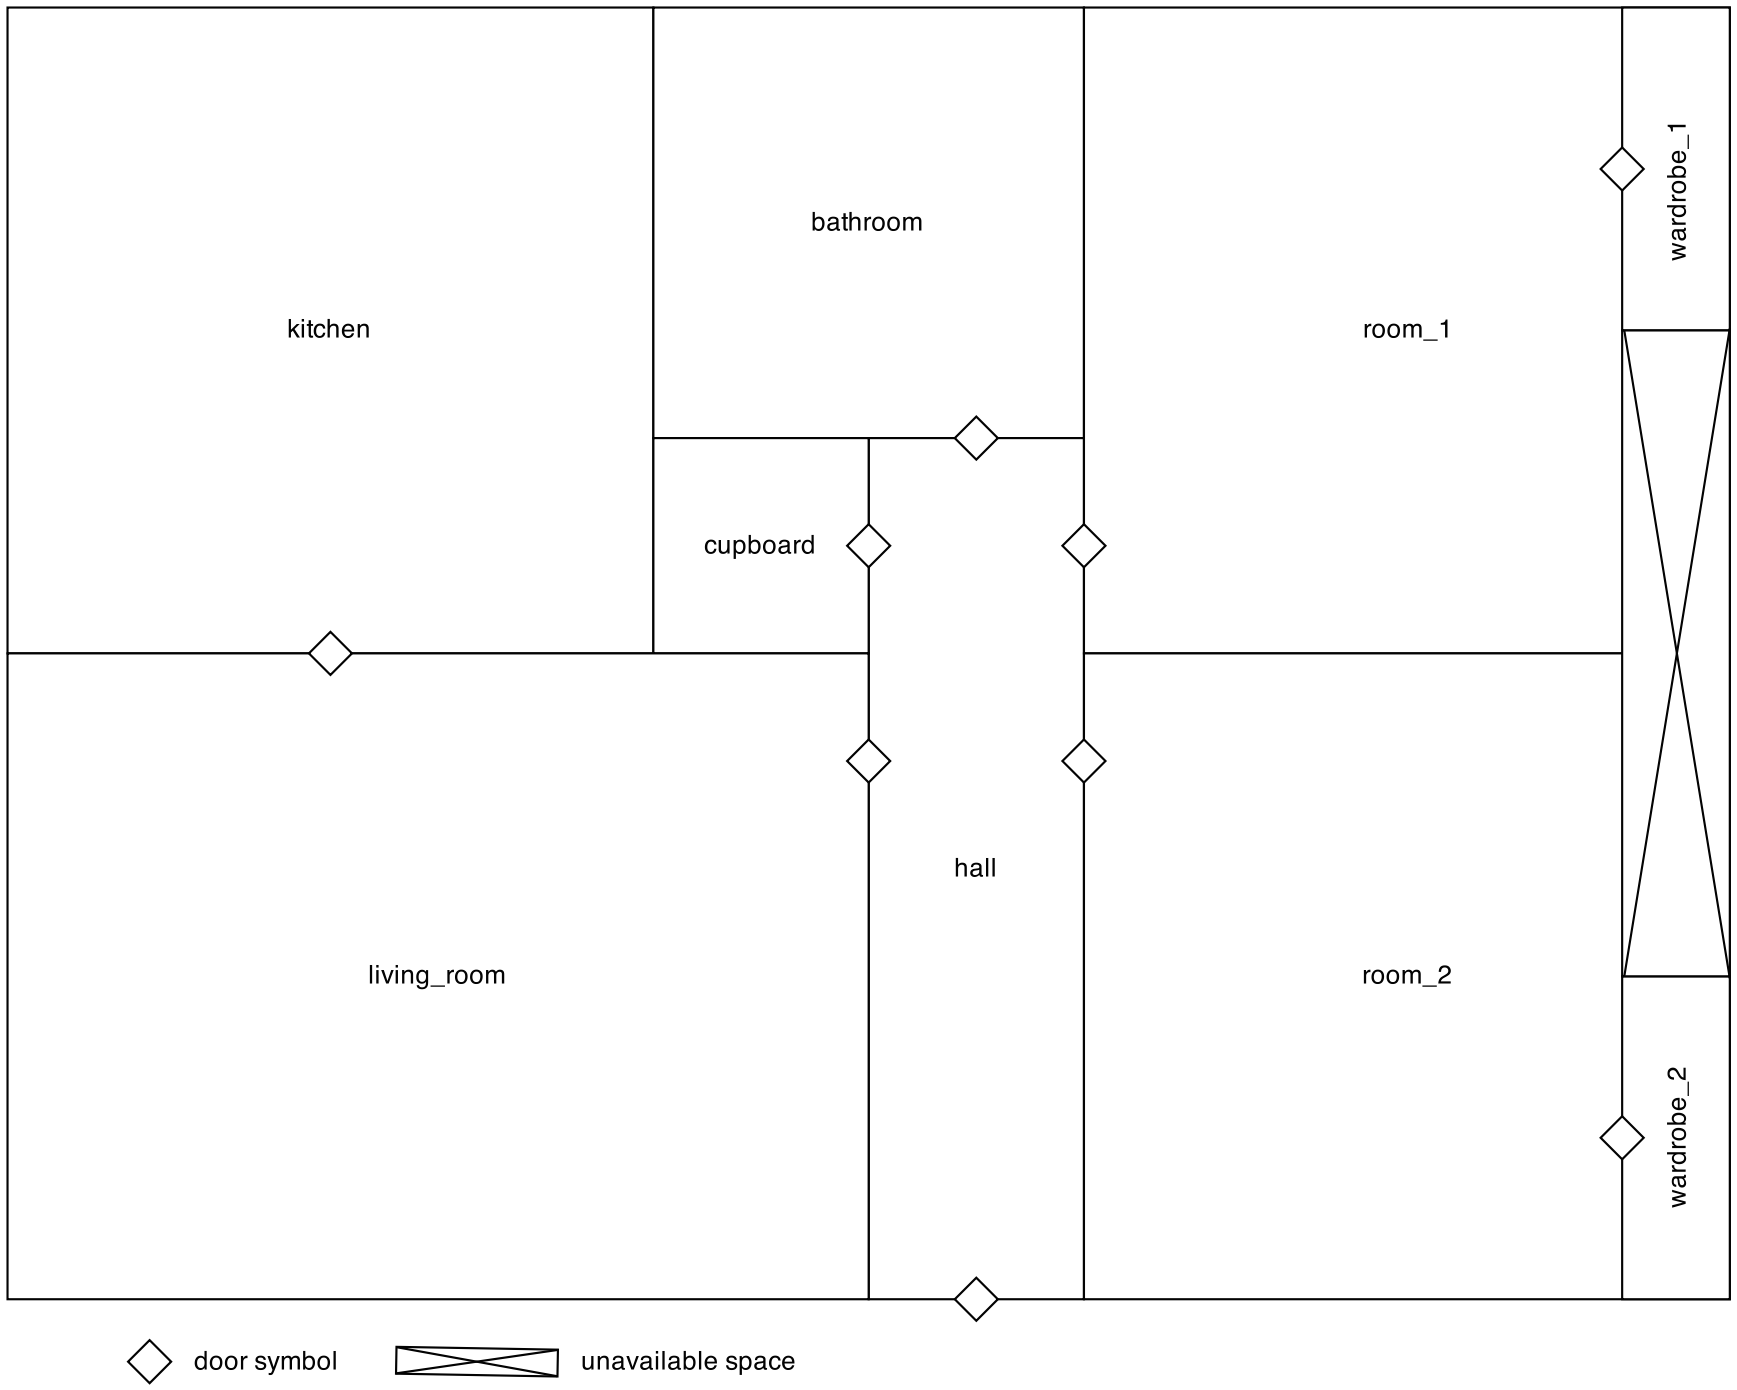
\includegraphics[height=7.3cm]{./gfx/room_layout}
  \caption{Simulated house room layout.\label{fig:simHouse}}
\end{figure}

    \subsection{Advantages}
Created smart house data generator is flexible and highly customisable. The simulated resident can perform tasks of arbitrary complexity ranging from simple motion to nested activities each using different combination of available items. Moreover, the output signals can be distorted with various kinds of noise and randomness.\\

The main advantage of proposed here simulation technique is detailed knowledge of the ground truth, which is based on the input activity script. Various kind of simulation statistics are available and can be used to visualise sensors behaviour, hence debug an activity model trained on the generated data.\\

Finally, the raw signal output of the generator is given in widely accepted CASAS format. Therefore, the simulations made with described here tool can be used together with all the activity recognition systems based on CASAS datasets.

    \subsection{ILP ready}
The smart house data generator is designed with the ILP model construction in mind, therefore it outputs \texttt{Prolog} facts needed for this purpose. Information such as the house specific background knowledge and positive \& negative examples required by the ILP algorithm are recorded.\\
Additionally, detailed sensors activations, time-location and activity structure informations are available for manual analysis of the output signals.

    \subsection{Proof of concept}
The value of presented here smart house data generator can increase significantly if it can be proven to produce real-like datasets. Proof for a single resident case is sufficient as a multiple residents house is based on combination of multiple single agent simulations. The latter is achieved by special handling (preserving sensors' states) of cases when the residents cross each other's paths and interact with common device or item.\\

Presented here data generator evaluation is based on \emph{similarity comparison} of the ILP models learnt on CASAS \#1 WSU Smart Apartment ADL Normal Testbed and synthetic datasets. The latter are generated based on as accurate CASAS testbed reproduction as possible. I chose this particular genuine data as they are provided with detailed activity scripts (see \emph{Section~\ref{sec:csasDataDet}}) and testbed layout (see \emph{Figure~\ref{fig:house:oner}}), hence its simulations should result in faithful reproductions.\\

To this end, I encoded CASAS testbed in my generator and simulated therein five described activities. I used all the features described in \emph{Section~\ref{sec:CASASflavour}} to learn the activity models.\\
For the synthetic data I was able to learn all the model rules presented in \emph{Figure~\ref{lst:CASASmodel}}. Due to noise present in the genuine CASAS data I was not able to learn all of the above activity rules for single trial (5 activities performed by one participant), nevertheless with large enough sample I could learn one rule at a time. Therefore, I conclude that within reasonable margin of error the generator produces real-like data.

  \section{Knowledge representation of spatio-temporal data}
The activity learning method described here requires signals to be represented as logical facts. The ILP system used in this study is written in \texttt{Prolog} programming language, therefore all the data has to be expressed in thereof predicates. This requirement causes some problems introduced by variety of used sensor types.\\

The most common sensor's output are binary variables: on-off, present-absent, opened-closed, etc.\ produced by motion, device and item sensors. Expressing them in logical form is straight-forward as their search space is finite---a set containing two elements. For convenience all binary variables are normalised to Boolean true-false space.

    \subsection{Unbounded sensor readings}
Another type of sensor's output are real and whole numbers. Handling these quantities is well known and broadly documented issue in artificial intelligence and logic programming. As \texttt{Prolog} is a language based on a search space traversal numbers i.e.\ unbounded variables, with their infinite (unbounded) search space are causing significant difficulties.\\

When the sensor's output is numerical it is converted into Boolean space by simple thresholding. The critical value is hand-picked based on observation of the sensor's output values.\\
A special case of unbounded readings is a time.

    \subsection{Time representation\label{sec:timeRepresentation}}
Date-time is a complex object encoding many useful information. Unfortunately, its human readable format---YYYY-MM-DD HH:mm:SS.ssssss---is of no use in computer science. Converted to machine language it is expressed as a \emph{timestamp}---number of seconds elapsed since epoch dated on 00:00:00, 1\ts{st} January 1970, UTC.\\

For my study I chose four different time representations:
\begin{description}
\item[absolute] is a timestamp represented in micro-seconds ($\mu$-seconds: $10^{-16}s$) rather than seconds,
\item[relative] is a number of micro-seconds elapsed since the first sensor activation in the dataset,
\item[sequence] is a sequential number of the sensor activation in the dataset starting with $0$,
\item[windowed] is a sequential number of fixed-time-interval window that the event falls into; the first time-window starts on the first sensor activation and has ID $0$; window of 5 seconds is used in the study.
\end{description}
Time representation examples are shown in \emph{Figure~\ref{lst:timerepresentation}}.\\

\begin{figure}[htb] % [breaklines]
  \begin{minted}[bgcolor=Bkgd,frame=leftline]{Prolog}
sensor(m12, true, relative, 4007842 ).
sensor(m12, true, absolute, 1430004781866056 ).
sensor(m12, true, sequence, 2 ).
sensor(m12, true, windowed, 0 ).

sensor(m13, false, relative, 5994214 ).
sensor(m13, false, absolute, 1430004783852428 ).
sensor(m13, false, sequence, 3 ).
sensor(m13, false, windowed, 1 ).
  \end{minted}
  \caption{Signal represented as \texttt{Prolog} facts.\label{lst:timerepresentation}}
\end{figure}

As no single time representation is the best for the ILP application all four were tested and evaluated. \emph{Sequence} is the most suitable in a search space environment---the numbers are not sparse, therefore the application can easily iterate through them without large computational overhead.\\
For this reason I chose this representation as the main time format. Despite being helpful in the ILP scenario sequential numbers are highly uninformative. They lack basic information such as time of day or possibility to be transformed into time elapsed since last sensor reading.\\

To enrich the source of information used by the learning algorithm \emph{timestamp} representation is used. Following directly from the sequential number it can be easily accessed. With such detailed representation of micro-second accuracy, precise time elapsed since any event can be calculated.\\
Moreover this value can be thresholded, hence discretised to produce bounded variables such as:
\begin{description}
\item[time of year] winter, summer, autumn, spring;
\item[month] January, February, March, etc.;
\item[time of day] morning, afternoon, evening, night;
\end{description}
and similar. In particular, in the ILP and AI such values are a lot easier to work with comparing to numbers.\\

The remaining two representations: \emph{relative} and \emph{windowed} are of little use in presented here learning approach.

    \subsection{Background knowledge\label{sec:data:bkg}}
Background knowledge is a general name for a place containing all the information relevant to the model learning. By far, it is the most important component of the ILP containing building blocks of the target model. Moreover, it is a place for logical representation of the signals and all relevant rules interacting with them. Additionally, it contains any information not given or implicit in the raw signals.\\

From a large enough sample of smart house data it is feasible to infer room layout and interconnections, unfortunately this task is computationally complex and impractical in most of the cases. The ILP comes with help in such scenarios as it is ready to use any information not given in the raw signal by reading it from its background knowledge file. Room connections information is a great feature as it helps to predict motion trajectory and person's location.\\
Sensor allocation---placement in the rooms---is another information not given in the raw signal. With help of sensors' location, motion sensors activations can be translated into the room name.\\
Examples of information used in the background knowledge file are given in \emph{Figure~\ref{lst:bg}}. Fact \texttt{connected} informs about the room connections via doors; \texttt{sensorInRoom} contains information where the sensor of given ID is placed; \texttt{sensorActivity} is used with all the item and appliance sensors and assigns human readable name to each sensor ID; finally, \texttt{sensorInField} tells in range of which motion sensor the item or appliance is located.\\

\begin{figure}[htb] % [breaklines]
  \begin{minted}[bgcolor=Bkgd,frame=leftline]{Prolog}
connected(     bathroom, hall    ).

sensorInRoom(  m61     , bathroom).

sensorActivity(ad1-c   , burner  ).

sensorInField( ad1-b   , m83     ).

aPriori(tv    , watchTV   ).
aPriori(burner, cook      ).
aPriori(phone , phone_call).

bedroom(residentA, bedroom1).
bedroom(residentB, bedroom2).
  \end{minted}
  \caption{Background knowledge facts snippet.\label{lst:bg}}
\end{figure}

Apart from house layout information \emph{prior believes} of any kind can be specified in the background knowledge---see \texttt{aPriori} keyword in \emph{Figure~\ref{lst:bg}}. A priori information such as likely place of activity, a device or item required to complete it, and the order of activities are of invaluable help. For example, watching TV is most often associated with being in the living room and a meal cannot be eaten unless it has been cooked. It is a fact that watching television requires TV to be on, cooking is happening with a hob on and to make a phone call one needs to use a phone.\\
With multiple residents in the house information such as bedroom assignment helps to distinguish them (\texttt{bedroom} keyword in \emph{Figure~\ref{lst:bg}}).\\

\begin{figure}[htb] % [breaklines]
  \begin{minted}[bgcolor=Bkgd,frame=leftline]{Prolog}
location(Time, Location) :-
  (sensorInRoom(SensorID, Location),
   sensor_state(SensorID, true, Time),
   Time >= 0, !  )
  ;( !, Time > 0,
    location(Time-1, Location) ).
  \end{minted}
  \caption{Example rule.\label{lst:bg:rule}}
\end{figure}

Another component of background knowledge are \texttt{Prolog} rules interacting with facts and signals---they can be understood as \emph{feature extractors}. Rule example is shown in \emph{Figure~\ref{lst:bg:rule}}; it queries \emph{where} (room name) a person is at given \emph{time}.\\

The background knowledge can be also understood as \emph{proxy} between the raw signals and high level activity rules. As the activity rules are based on room, item, appliance names and not sensor IDs they are universal. Therefore, already existing model can be applied to any other house by using specific to that residence background knowledge.\\
Finally, learnt rules can be used in future iterations of learning process by appending them to the background knowledge file.


    \subsection{Positives and negatives\label{sec:data:posneg}}
The final component of the ILP are positive and negative examples of the target model. Sample facts for both single and multiple residents are presented respectively in \emph{Figure~\ref{lst:singleposneg}}~\&~\emph{\ref{lst:multiposneg}}.\\

\begin{figure}[htb] % [breaklines]
  \begin{minted}[bgcolor=Bkgd,frame=leftline]{Prolog}
activity(cook  , 47).
activity(eat   , 51).
activity(eat   , 52).
activity(eat   , 53).
activity(washUp, 59).
activity(washUp, 60).
  \end{minted}
  \caption{Positives and negatives for single resident.\label{lst:singleposneg}}
\end{figure}

These examples use \emph{sequence} representation of time to express when (and by whom) activity \emph{is}---positives, and \emph{is not}---negatives done. Both types have a common structure and are separated into two different files to be distinguishable.\\

\begin{figure}[htb] % [breaklines]
  \begin{minted}[bgcolor=Bkgd,frame=leftline]{Prolog}
activity(sleep, 14, residentA).
activity(sleep, 15, residentA).
activity(sleep, 16, residentA).
activity(sleep, 17, residentA).
activity(useBathroom, 4, residentB).
activity(useBathroom, 5, residentB).
activity(useBathroom, 6, residentB).
activity(useBathroom, 7, residentB).
  \end{minted}
  \caption{Positives and negatives for multiple resident.\label{lst:multiposneg}}
\end{figure}

For each activity the sets of positive and negative examples have to be disjoint with regard to the time---see \emph{Figure~\ref{fig:timepoints}} for reference. The ILP system generalises positive examples into complex rules---containing feature predicates in their body---under restriction of not covering any or majority of negative examples.

  \section{The converter}
The next step in model learning is data conversion from CASAS-like log format to \texttt{Prolog} \emph{knowledge representation} i.e.\ state signal readings as logical facts. The converter is capable of handling both single and multiple residents datasets. To this end, a number of conversion steps is need.\\

Real-valued signals like AD1-B water sensor (see \emph{Figure~\ref{lst:CASASoneR}}) are threshold and discretised. Binary sensor's outputs are unified to values \emph{true} and \emph{false}. The time-date information is converted into four described in \emph{Section~\ref{sec:timeRepresentation}} representation.\\
Moreover, the converter uses activity and person ID information given in the 4\ts{th} and 5\ts{th} column of the data to generate positive and negative examples needed for learning activity model with \texttt{Aleph}.

  \section{Cross-validation}
Once the data is converted and passed to \texttt{Aleph} the model in form of a rules describing activities is produced. To evaluate its quality 10 fold cross-validation is performed.\\
For each experiment 10 data recordings are gathered together with corresponding activity models learnt with the ILP. The genuine data are split per trial to create folds. For the synthetic data 10 independent recordings are produced each varying in the inhabitant's path and order of used items.\\
Then, each sample model is evaluated on the remaining nine datasets and the results are checked against the corresponding ground truth information. After testing all possible model-data combinations overall and per-label confusion matrices are reported. The output of cross-validation framework is one of the diagnostics used to evaluate the model performance.

  \section{Summary}
In this chapter I familiarised myself with the real smart house data. I also identified their issues and decided to design a smart house data generator to mitigate from them and focus on the model learning task. Moreover, I settled on a numerical-valued sensor handling and identified the most suitable time representations for the ILP learning. Additionally, I examined relevant domain specific background knowledge for the smart house data, which proved to be invaluable in the model learning. Finally, I designed scripts to convert CASAS formatted data into logical fact representation; perform cross-validation on learnt models; and variety of supplementary \texttt{Bash} and \texttt{Python} scripts to make the data handling and model learning easier.\\
The next component of my work is to discover details of the ILP learning and adjust it to activity recognition task.

%===============================================================================
%===============================================================================
%===============================================================================
%===============================================================================
%===============================================================================
\chapter{Inductive Logic Programming\label{ch:ILP}}
\citet{plotkin1972automatic} in early 1970s and \citet{shapiro1983algorithmic} in early 1980s created foundation of the \emph{Inductive Logic Programming} (ILP). Both authors introduced techniques and tools to learn \emph{first-order formulas} (parametrised rules that are the core of the ILP) describing chosen object based on a set of facts. Since then, the ILP techniques found number of interdisciplinary applications with new rule learning tools being created now and then.

  \section{Inductive Logic Programming}
The concept of the inductive logic programming is based on fusion of two well known techniques: \emph{inductive learning} and \emph{logic programming}. The first component facilitates building model from available observations and generating new knowledge form experience. The latter, introduces a powerful representation of knowledge as \emph{first-order logical rules}~\citep{muggleton1994inductive,muggleton1995inverse}.

    \subsection{Logic programming}
\emph{Propositional logic} widely used in machine learning models is strictly ``\emph{weaker}'' than \emph{first-order logic} used in the ILP. A propositional sentences (rules) are made of facts combined with \emph{logical connectives} such as: not ($\neg$), and ($\land$), or ($\lor$), existence ($\exists$), etc.. Such sentence can only be evaluated to true or false based on predicates in its body e.g.\
$$\left(\left(\texttt{sensorM42} \land \texttt{sensorM47}\right) \lor \left(\texttt{sensorM27} \land \texttt{sensorM30}\right)\right) \land time = 40$$
where \texttt{sensor$\Bigcdot\Bigcdot\Bigcdot$} denotes sensor $\Bigcdot\Bigcdot\Bigcdot$ being on. The above sentence is true if either both \texttt{sensorM42} and \texttt{sensorM47} or \texttt{sensorM27} and \texttt{sensorM30} are simultaneously on at time $40$.\\

Thanks to first-order logic the ILP overcomes presented above ``limited representation formalism''---expressing data in form of a propositional logic. Many problems considered hard to solve while expressed propositionally can be easily tackled with the ILP. The power of first-order logic lies in expressing its sentences with \emph{parametrised} predicates. Use of domain specific quantified variables alters logical state of the sentence based on inputs and outputs of its predicates, therefore facilitates expressing complex relations. An example of first-order activity rule: \texttt{activity(A,B)} where variable \texttt{A} denotes activity ID and \texttt{B} time, is given below. The rule illustrates the dependencies between predicates via free variable \texttt{C}.
\begin{eqnarray*}
&\texttt{activityOrder(B,A)} \land \texttt{location(B,livingRoom)} \land \\
&\texttt{outOfCabinet(B,C)} \land \texttt{medicineInList(C)}
\end{eqnarray*}
The major limitation of first-order logic is its restriction to finite variable domains---it cannot describe rules built on infinite sets like real or natural numbers.\\

Finally, the ILP does not have difficulties in incorporating substantial background knowledge in form of a first-order sentences to the model. This feature is not very common among other machine learning models, nevertheless use of domain knowledge is ``essential for intelligent behaviour''~\citep{muggleton1994inductive}.

    \subsection{Inductive learning}
The second component of the ILP is inductive learning: constructing \emph{first-order clausal theories}. Such hypotheses are based on combining background knowledge with facts representation of positive and negative examples; see \emph{Figure~\ref{fig:ilp}}.\\
\begin{figure}[htb]
  \centering
  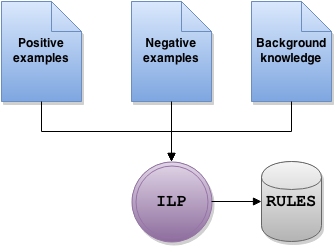
\includegraphics[scale=.5]{./gfx/ilp}
  \caption{ILP scheme\label{fig:ilp}}
\end{figure}
ILP aims at building theory that under consideration of background knowledge explains facts: covers as much positive examples as possible without covering and or most of negative examples. To this end, it uses \emph{induction} as a basic mode of inference: generalization of specific observations to theories, rather than deduction: transforming general theories to the more specific clauses.

    \subsection{Applications}
The rules produced with the ILP are human readable (unlike models generated by majority of other machine learning solutions) what gives it great advantage over competition. Easy to understand rules means that the logical models are arguably easy to manipulate. They can be changed by simply adding, deleting, and modifying clauses or literals.\\
Such model representation is invaluable in \emph{scientific theory formation} and problems where data cannot be easily represented in attribute-vale language. The ILP is widely used in structure-activity prediction for drug design~\citep{king1992drug,michael1992modelling} and protein secondary-structure prediction~\citep{muggleton1992protein}. It is also a popular tool in computer science used for: programming assistance, algorithmic debugging, program testing and verification, and reverse engineering~\citep{shapiro1983algorithmic,bergadno1993inductive,bratko1993inductive}.\\

The two most popular \texttt{Prolog} ILP implementations are \texttt{Aleph}\footnote{\url{http://www.cs.ox.ac.uk/activities/machlearn/Aleph/aleph.html}} and \texttt{Progol}\footnote{\url{http://www.doc.ic.ac.uk/~shm/progol.html}}. \texttt{Aleph} is chosen for this study due to its comprehensive documentation and ease of use on contemporary platforms.

  \section{\texttt{Aleph}}
\texttt{Aleph}: A Learning Engine for Proposing Hypotheses, is \texttt{Prolog} based Inductive Logic Programming system developed at Oxford University by \citeauthor{muggleton1994inductive}. It is compatible with two most popular \texttt{Prolog} language implementations: \texttt{YAP}---Yet Another Prolog, and \texttt{SWI-Prolog}.

    \subsection{Input files}
\texttt{Aleph} infers hypotheses using three files, the first two contain positive and negative examples of the target rule model, the third encodes program settings and any additional informations.

      \subsubsection{Background}
The background file contains \texttt{Aleph} configuration and a target model specification; see example given in \emph{Figure~\ref{lst:alephSettings}}. Settings such as evaluation function, allowed maximal number of negative examples covered by a single target rule, and minimal number of positive examples that each rule has to cover are used.\\

Additionally, the target rule specification has to be provided. Based on presented here example the target \texttt{activity} rule has $2$ variables (is of \emph{arity} $2$) and its body can contain arbitrary number of \texttt{device} and \texttt{location} predicates each of arity $2$---\texttt{determination} settings.\\
Next, the types of the variables for each predicate has to be specified. \texttt{modeh} and \texttt{modeb} determine structure of the target rule \emph{head} and \emph{body} respectively. Both mode declarations set:
\begin{itemize}
\item a number specifying successful calls to the specified predicate or a * symbol to set bounded non-determinacy\footnote{See \texttt{Aleph} manual for detail: \url{http://www.cs.ox.ac.uk/activities/machlearn/Aleph/aleph.html}};
\item a name of the predicate to be called, together with its variables types specification.
\end{itemize}
By large, the modes define how to call the target rule and the predicates used in its body; they set whether variables should be an input (a + symbol); an output (a - symbol); or a constant (a \# symbol).\\

In presented here example the \texttt{activity} rule takes constant activity ID and input integer representing time. Both \texttt{device} and \texttt{location} predicated take time as their first input variable. Additionally, the first takes constant device ID and the latter room ID.\\
Each variable type needs to be specified as an exhaustive set represented in logical facts. In presented here example the activity ID can be either \texttt{wash\_hands} or \texttt{clean}, the device ID can be either \texttt{phone} or \texttt{hot\_water} and the room ID can be either \texttt{hall} or \texttt{kitchen}.\\
Finally, the target model constrains can be specified with \texttt{false} keyword: in presented example no two different activities can happen at the same time.\\

\begin{figure}[htb] % [breaklines]
  \begin{minted}[bgcolor=Bkgd,frame=leftline]{Prolog}
% Internal settings
:- set(evalfn, wracc).
:- set(noise , 3    ).
:- set(minpos, 1    ).
% Determinations
:- determination(activity/2, device/2  ).
:- determination(activity/2, location/2).
% Mode declarations: rule head definition
:- modeh(*, activity(#activityIDs, +integer) ).
% Mode declarations: rule body definition
:- modeb(*, device(+integer, #deviceIDs)).
:- modeb(*, location(+integer, #roomIDs)).
% Type specification
activityIDs(wash_hands).
activityIDs(clean     ).
deviceIDs(phone    ).
deviceIDs(hot_water).
roomIDs(hall   ).
roomIDs(kitchen).
% Constrains
false :-
  activity(Activity1, T),
  activity(Activity2, T),
  not(Activity1 = Activity2).
  \end{minted}
  \caption{Example \texttt{Aleph} settings.\label{lst:alephSettings}}
\end{figure}

Therefore, target rules are of the form \texttt{activity(ActivityID, Time) :- $\Bigcdot$}.\\

Additionally to presented above \texttt{Aleph} settings, background knowledge file also contains domain specific facts and rules discussed is \emph{Section~\ref{sec:data:bkg}}.

      \subsubsection{Positives}
Positive examples file lists activity facts of the form \texttt{activity(ActivityID, Time).} to indicate at which time points the activity was happening in the data. Example file is discussed in \emph{Section~\ref{sec:data:posneg}}.

      \subsubsection{Negatives}
Negative examples file is of the same form as the positive example file. It indicates time-points when activities were not undertaken. In presented here learning scenario the negative time-points are set complement of the positive examples and are bounded from below by $0$ and from above by the number of sensor readings in the dataset; see \emph{Figure~\ref{fig:timepoints}} for reference. Example file is discussed in \emph{Section~\ref{sec:data:posneg}}.

\begin{figure}[htb]
  \centering
  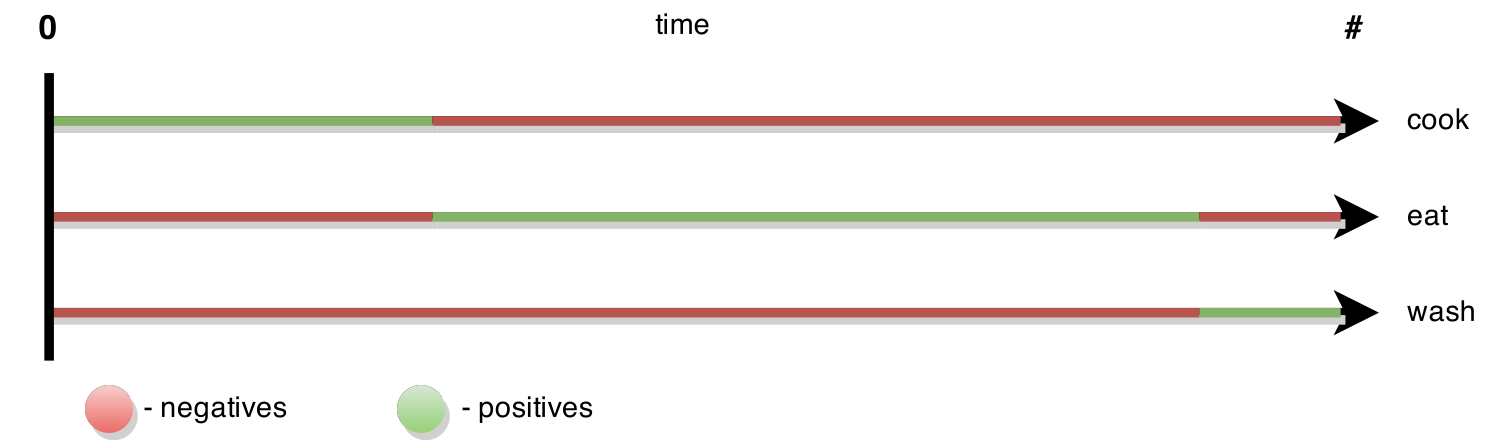
\includegraphics[width=.85\textwidth]{./gfx/activityStructure}
  \caption{Activity structure example.\label{fig:timepoints}}
\end{figure}

    \subsection{\texttt{Aleph} output}
Based on the input data \texttt{Aleph} outputs set of rules compliant with given specification. Presented in \emph{Figure~\ref{lst:alephSettings}} settings could result in the first from the top rule given in \emph{Figure~\ref{lst:alephOut}}. It does not contain free variables in the body hence can be expressed in propositional logic.\\
The second one is more complex yet still propositional. \texttt{outOfCabinet(A,[none])} predicate gives list of items taken out of cupboard at time \texttt{A}.\\
The third activity rule is a \emph{singularity}. Positive example \texttt{activity(clean,87).} is outputted as the ILP algorithm could not generalise it to a proper rule without breaking any of the restrictions imposed by the background file. Such rules are pruned out prior to cross-validation.\\

\begin{figure}[htb] % [breaklines]
  \begin{minted}[bgcolor=Bkgd,frame=leftline]{Prolog}
activity(wash_hands,A) :-
  device(A,water_hot).

activity(wash_hands,A) :-
  outOfCabinet(A,[none]),
  waterUsed(A).

activity(clean,87).
  \end{minted}
  \caption{Example activity model.\label{lst:alephOut}}
\end{figure}

An example of more advanced, first-order logical rule is presented in \emph{Figure~\ref{lst:bg:rule}}. Free variables present in the rule body ensure interaction between clauses.

    \subsection{The basic algorithm}
In general, the inductive logic programming is a \emph{search problem}. The algorithm traverses through \emph{candidate solution space} i.e.\ set of ``well-formed'' hypotheses, to find the most suitable one. The ILP problem can be solved using a na\"{\i}ve generate and test algorithm, however, this approach is highly inefficient. The most suitable solution has four steps: select example, build most-specific-clause, search, and remove redundancies~\citep{muggleton1994inductive}.

      \subsubsection{Select example}
Select a positive example form the positives set that is not yet covered by learnt rules. If all positives are tested stop the procedure.

      \subsubsection{Build most-specific-clause}
Also known as the \emph{saturation step}. Construct a \emph{bottom clause}: definite clause with many literals that is most specific given that it entails previously selected example and complies with provided restrictions.

      \subsubsection{Search}
Also known as the \emph{reduction step}. Search through subsets of previously found literals to build more general clause that complies with given restrictions. A more general clause can improved performance by covering more than one positive example.

      \subsubsection{Remove redundancies}
Also known as the \emph{cover removal}. Memorise the clause with the best score (coverage) and remove positive examples made redundant (covered) by the new clause. Finally, return to \emph{select example} step.

  \section{Applications to spatio-temporal data}
With a bit of tuning the ILP can be applied to any spatio-temporal data with quite good results. Despite difficulty with handling numerical values rule based model is highly suitable for the activity recognition task.\\

Arbitrary information that can be appended to the background knowledge greatly improves raw signal handling. \texttt{Prolog's} \emph{negation as failure} is consistent with commonly lacking sensor states. \texttt{Prolog} assumes that any sensor is off if it cannot be ``proven'' to be on; regardless of whether it does not exist at all or it has not been activated yet, hence, according to the data it is neither on nor off. This approach helps in smoothing out sensor readings e.g.\ if current location cannot be inferred from available sensor readings the model assumes last known location (see \emph{Section~\ref{sec:predictionDiscontinuity}}).\\

Moreover, the output model written in \texttt{Prolog} is human readable, therefore relations in the data revealed by the ILP can be understood and used to improve the model. The output theory can be also easily modified and enclosed within meta-rules. This practice is an easy fix for prediction discontinuity issues; see \emph{Section~\ref{sec:predictionDiscontinuity}} for details.\\

Finally, expressing hierarchy in the rule based model can be easily achieved by placing one rule in the body of the other or conditioning only on some subset of the rule body literals. The concepts of rule generalisation and specialisation directly correspond to moving up and down the hierarchical structure.

  \section{Closed Concept \& Least General Generalisation\label{sec:closedConcept}}
A \emph{closed concept} is a concept that includes all implicitly understood conditions. For example rule:\\
\begin{minted}[bgcolor=Bkgd,frame=leftline]{Prolog}
activity(wash_hands,A) :-
  device(A,water_hot),
  location(A,kitchen).
\end{minted}
and:\\
\begin{minted}[bgcolor=Bkgd,frame=leftline]{Prolog}
activity(wash_hands,A) :-
  device(A,water_hot).
\end{minted}
both have the same coverage of positive examples, but the first is more specific, therefore it is a closed concept. In other words, it is the \emph{least general generalisation} (LGG) of chosen positive example.\\

Due to \texttt{Aleph's} search step, bottom clause i.e.\ LGG of currently selected positive example, is pruned of redundant (from performance perspective) literals, hence activity details are lost. In the example given above location of washing hands is reduced. These disregarded informations are of great importance for feature construction and data narrative (see \emph{Section~\ref{sec:narrative}}).\\

It is possible to generate closed concept of activity rules in \texttt{Aleph} by disabling search step. To achieve this, the search setting has to be overwritten: \texttt{:- set(search, false).}~.

  \section{Feature discovery and feature extraction}
Building a data model with the ILP requires right features to be available in the background knowledge file. By large, the ILP algorithm searches through feature space to find their most suitable combination for each activity rule. In presented here scenario features are understood as rules interacting with raw signals, domain specific background knowledge and each other in order to extract information relevant to the model.\\
Designing such rules can be understood as feature construction and requires awareness of ``activity script'' used to generate the data regardless of their origin: simulation or experiment participant interacting with a smart house. The ``activity script'' can be both: general description of activities or ordered list of tasks to be perform by a participants. If such script is not available, a careful data analysis is required prior to feature construction.\\

Additionally, the rule body of outputted activity model can be examined to analyse relations between features and activities. Interesting predicates can be then applied directly to the raw dataset to generate new feature vectors. It is widely known that well crafted features can boost performance of any machine learning model. Moreover, more informative LGG of the output rules can be checked.\\
Features used for both single and multiple residents models are discussed in detail in \emph{Section~\ref{sec:single:features}}.

  \section{Summary}
In this chapter I showed that the concept of Inductive Logic Programming can be adapted to serve as a tool for building the activity recognition models. Moreover, I explained that the ILP is capable of comprehensive data analysis, hence feature discovery, by outputting human readable closed concept of each positive activity example.\\
Additionally, I outlined the basic internals of the ILP mechanism together with \texttt{Aleph} settings useful for the model learning. Finally, good understanding of the smart house data and all the aforementioned ILP components opened up the possibility to learn fully featured activity recognition models.


%===============================================================================
%===============================================================================
%===============================================================================
%===============================================================================
%===============================================================================
\chapter{Activity recognition model}
The activity recognition model predicts agent's \emph{actions} at \emph{time} of interest based on signals delivered by a smart house. Therefore, the target rule needs an input variable \texttt{Time} and output variable \texttt{Activity} leading to:\\
\begin{minted}[bgcolor=Bkgd,frame=leftline]{Prolog}
activity(Activity, Time) :-
  ruleBody.
\end{minted}
and for a multiple residents houses another output variable to predict a \texttt{Person} performing the activity is necessary:\\
\begin{minted}[bgcolor=Bkgd,frame=leftline]{Prolog}
activity(Activity, Time, Person) :-
  ruleBody.
\end{minted}
The \texttt{ruleBody} is made of rules encoded in the background knowledge which serve as features. They extract relevant informations form the house signals.

  \section{Scripted data} % WHY I chose this that and that!!!!!!!!!!!!
As the rule format is determined, the next step it to design the features contributing to the rule body. To this end, an insight into how to distinguish particular activities is needed. Scripted CASAS datasets (see \emph{Section~\ref{sec:csasDataDet}}) are of great help. Their careful analysis can reveal patterns that can be used to differentiate the activities.
% by their careful examination

    \subsection{Sequential multi-class model for single resident\label{ch:smcm}}
Beside the target rule specification, the model assumptions need to be stated. Based on CASAS scripted data it is clear that activities are sequential and that they do not overlap (see \emph{Figure~\ref{fig:timepoints}}). Hence, the problem is single-label and \emph{multi-class}---there is always one label to be assign to a time point and this label is chosen from a set which usually has cardinality greater than 2.

    \subsection{Basic activities\label{sec:basicActibities}}
To start model learning I selected two activities: \emph{cook} and \emph{phone call}, and generated my impression of them for one resident based on CASAS description. Therefore, the resulting synthetic dataset is simple, completed, noiseless and resemble real life activities. Such a simple learning task helped me to familiarise myself with \texttt{Aleph} data analysis mechanisms and discover its basic capabilities and limitations.

      \subsubsection{Encode activities}
I decided to script a simple scenario in the house given in \emph{Figure~\ref{fig:simHouse}}. A person starts in the hall with a random location; he moves to the living room; activity \emph{phone\_call} starts; he approaches the phone book (finds a phone number); he moves to the fixed phone (talks for some time); activity \emph{phone\_call} ends. Then the person goes to the kitchen; the activity \emph{cook} starts; he approaches and uses hob for some time; the activity stops when he turns off the hob. Finally, the person goes back to the hall via the living room.\\

The detailed knowledge of steps taken by the resident allows to design basic features and test them. The data produced by the generator are in CASAS log format, therefore they are converted into a facts representation. Then, the logical signal representation is joined with the house specific facts to produce basic background knowledge file. Additionally, during conversion step positives and negatives are produced. Hence, all the basic components for the ILP learning are present.

      \subsubsection{Design features}
In order to build the activity model needed feature rules have to be added to the background knowledge file. Based on the script used to generate the data I know that both activities can be distinguished by the \emph{location}: phone call happens in the living room and cooking in the kitchen. Moreover, for both activities different devices and items are used: for the first the phone book and the fixed phone; for the latter the hob.\\

Therefore, this simple model should work with just these two features. The basic building block of both of them is a \texttt{Prolog} predicate which interacts with sensors readings. It finds activated sensor at given time via input/output variable \texttt{SensorID}, input/output variable \texttt{SensorState} and input variable \texttt{Time}. As there are multiple time representation additional input/output \texttt{TimeType} variable is needed to represent them leading to the rule of the form:\\
\begin{minted}[bgcolor=Bkgd,frame=leftline]{Prolog}
sensor_state(SensorID, SensorState, TimeType, Time) :-
  ruleBody.
\end{minted}
For simplicity, in my activity recognition model the input \texttt{Time} and input/output \texttt{SensorID} variables suffice. Through the task only the \emph{sequential} time representation is used and the \emph{activated} sensors are of interest. Therefore, the above rule can be wrapped to provide a simple interface to the sensors state information:\\
\begin{minted}[bgcolor=Bkgd,frame=leftline]{Prolog}
sensor_state(SensorID, Time) :-
  sensor_state(SensorID, true, sequence, Time).
\end{minted}
Presented here rule is highly customisable as it facilitates selection of the time representation and allows to condition on deactivated sensors if needed.\\

All the \texttt{Prolog} rules are built by logical constrains warranting correct answer. For the \texttt{sensor\_state} rule to be true, the sensor \texttt{SensorID} had to be activated at latest at the time \texttt{Time}, and after its activation (but before time \texttt{Time}) the \texttt{SensorID} had not been deactivated. These two conditions guarantee correct sensor status checks.\\
Moreover, as \texttt{Prolog} uses a search space to ``answer'' queries rule variables can be both input and output. If all variables are initialised i.e.\ they are used as an input, the rule is used to check correctness of the believes and evaluates either to \texttt{true} or \texttt{false}. If the rule contains some uninitialised variables \texttt{Prolog} can find their unifications that yield \texttt{true} evaluation of the rule; it is worth to mention that multiple results can be returned.\\

The \texttt{sensor\_state} rule covers both \emph{item} and \emph{motion sensor}. It is worth separating the two aforementioned cases to improve the model clarity. With use of house-specific background knowledge motion sensor IDs can be associated with rooms and item sensor IDs with devices and items.\\
Therefore, the device rule can be easily constructed as:\\
\begin{minted}[bgcolor=Bkgd,frame=leftline]{Prolog}
device(Time, Device) :-
  sensor_state(SensorID, Time),
  sensorActivity(SensorID, Device).
\end{minted}

The location rule could be created in a similar manner, i.e.:\\
\begin{minted}[bgcolor=Bkgd,frame=leftline]{Prolog}
location(Time, Location) :-
  sensor_state(SensorID, Time),
  sensorInRoom(SensorID, Location).
\end{minted}
Unfortunately, this simplification causes \emph{discontinuous} location predictions. To fix it, a case when none of the motion sensors is activated needs to be covered. By introducing a small bias and using the last known location (self-recursion with decreasing time) if none can be predicted a continuous prediction is ensured.\\

Finally, all three rules have to be appended to the \texttt{Aleph}'s background knowledge file to be used in the learning process.

      \subsubsection{Configure \texttt{Aleph}}
Both \texttt{location} and \texttt{device} features presented above are used to build the first activity recognition model. To this end, \texttt{Aleph} needs to be correctly configured.\\
The most important settings are \texttt{noise} and \texttt{minpos} parameters. These values are set to $5$ and $1$ respectively. The first is based on observational studies, and the latter is the lowest acceptable value so that every possible activity rule can be discovered. Unfortunately, setting \texttt{minpos} to $1$ results in many singleton rules---copies of the positive examples---appearing in the output theory; to remove them additional script is used after the learning step.\\

The next type of settings determines parameters of the target model. \texttt{determination}s indicate that both \texttt{device} and \texttt{location} predicates can contribute to the target rule body. \texttt{mode}s specify types of variables accepted by each predicate. The types of variables are declared in the house specific background knowledge.\\

The \texttt{Aleph} settings used to train this model are presented in \emph{Figure~\ref{lst:alephConfHead}}. Other than the aforementioned settings are left default.\\

\begin{figure}[htb]
  \begin{minted}[bgcolor=Bkgd,frame=leftline]{Prolog}
:- set( noise,  3 ).
:- set( minpos, 1 ).

:- determination( activity/2, device/2   ).
:- determination( activity/2, location/2 ).

:- modeh( *, activity(#activityIDs, +integer) ).
:- modeb( *, device(+integer, #deviceIDs)     ).
:- modeb( *, location(+integer, #roomIDs)     ).
  \end{minted}
  \caption{\texttt{Aleph} configuration header.\label{lst:alephConfHead}}
\end{figure}

Finally, the last step before running the algorithm is attaching the \texttt{Aleph} configuration together with house specific facts, feature rules, and smart house signals to the background knowledge file.

      \subsubsection{Learn the model}
As the \texttt{Aleph} learning process is interactive a special script is designed to improve the work-flow. The script runs the \texttt{Aleph}, loads all needed files: background, positives and negatives; learns the activity theory; and finally saves it to a file.\\
Then, the model is purified by removing singleton rules and retaining the ones with non-empty body. The resulting model is presented in \emph{Figure~\ref{lst:alephBasicModel}}.\\

\begin{figure}[htb]
  \begin{minted}[bgcolor=Bkgd,frame=leftline]{Prolog}
activity(phone_call,A) :-
  device(A,phone_book).
activity(phone_call,A) :-
  device(A,phone).
activity(cook,A) :-
  device(A,burner).
  \end{minted}
  \caption{Basic activity recognition model.\label{lst:alephBasicModel}}
\end{figure}

The learnt rules make perfect sense with regard to the activity script used to generate the data. Moreover, identified and encoded features behave as intended extracting relevant information from the smart house signal. Finally, the \texttt{location} feature does not appear in the model as it is uninformative in this case---see \emph{Section~\ref{sec:closedConcept}} for details.

      \subsubsection{Evaluate the results}
The activity recognition model built with presented above components is rather simplistic: it uses only one feature---see \emph{Figure~\ref{lst:alephBasicModel}}.\\

To evaluate the performance of the above model I use 10 folds cross-validation. Each fold is generated according to the same activity script but with a small variations in the resident's path. To fix the prediction discontinuity problem and improve the classification results a meta-rule proposed in \emph{Section~\ref{sec:predDis}} is used. The cross-validation results are presented in \emph{Figure~\ref{tab:basicStats}}.\\

\begin{figure}[htb]
  \centering
  \begin{tabular}{ c r | l l l r }
\multicolumn{2}{c}{} & \multicolumn{3}{c}{\emph{Predicted}} \\
 & & \textbf{cook} & \textbf{phone\_call} & \textbf{none}\\
\cline{2-5}
% \parbox[t]{2mm}{\multirow{3}{*}{\rotatebox[origin=c]{90}{rota}}}
\multirow{3}{*}{\rotatebox[origin=c]{90}{\emph{Actual}}}
% \multirow{3}{*}{\emph{Actual}}
 & \textbf{cook} & $\mathbf{87}$ & $\mathbf{4}$ & $\mathbf{0}$ & 91\\
 & \textbf{phone\_call} & $\mathbf{0}$ & $\mathbf{102}$ & $\mathbf{14}$ & 116\\
 & \textbf{none} & $\mathbf{26}$ & $\mathbf{7}$ & $\mathbf{48}$ & 81\\
\multicolumn{2}{c}{} & 113 & 113 & 62 & 288\\
  \end{tabular}
  \caption{Cross-validation results.\label{tab:basicStats}} % 91/288*0.96+116/288*0.88+81/288*0.59
\end{figure}

Overall, the model achieves \emph{accuracy} of \textbf{82.29\%}. Per-class \emph{precision} and \emph{recall} are: for the cooking \textbf{0.77} and \textbf{0.96}; for the phone call \textbf{0.9} and \textbf{0.88}; and for none activity \textbf{0.77} and \textbf{0.59}. The overall precision and recall can be calculated as a weighted average of the above taking the class proportion into account, hence \textbf{0.82} and \textbf{0.82}. Therefore, the overall \emph{F-measure} is \textbf{0.82}.\\

These results can be compared with baseline achieved by predicting the majority class. Such classifier achieves accuracy of \textbf{40.28\%}, with overall \emph{precision} of \textbf{0.16} and \emph{recall} of \textbf{0.40} yielding \emph{F-measure} of \textbf{0.23}.\\

Comparing both activity recognition models indicates that the rule based classification is superior to the majority class prediction in this simple scenario. Analysis of the confusion matrix and the model reveals that majority of the false predictions are caused by lack of informative features in the data, hence last known activity is predicted---see \emph{Section~\ref{sec:predictionDiscontinuity}}.\\

With comprehensive analysis of the ILP application to the basic smart house data I proceed to a more difficult case. All further model evaluation is based on proposed here framework.

    \subsection{CASAS flavoured activities\label{sec:CASASflavour}}
The next step is to reproduce CASAS \#1 WSU Smart Apartment ADL Normal Testbed scripted data presented in \emph{Section~\ref{sec:csasDataDet}} as faithfully as possible. The main difference is complete lack of noise to make feature design and extraction easier.

      \subsubsection{CASAS features}
The main advantage of this dataset is an activity script explaining step-by-step actions contributing to the five monitored activities. To design features capable of classifying these activities I identified their characteristic features.\\

The phone call uses two specific to this activity items: the phone book and the fixed phone. Therefore, this activity can be identified using previously designed \texttt{device} feature. The phone call rules are the same as the ones shown in \emph{Figure~\ref{lst:alephBasicModel}}.\\

The hand washing activity requires use of water. Moreover, unlike in cleaning and cooking tasks all the items stored in the cupboard are in place. These observations lead to two new features: \texttt{waterUsed(T)}---which checks whether at time $T$ either hot or cold water is used; and \texttt{outOfCabinet(T, ItemList)}---which finds items missing from the cupboard at time $T$.\\

The next activity recorded in the CASAS dataset is cooking. The first possibility to identify this activity is hob being on---it can be detected with \texttt{device} feature.\\
The second is based on past observations. The streaming scenario of a smart house data allows to use past activity predictions as a feature. In CASAS data cooking can be predicted if some items are removed from the cupboard and the resident has not been cooking in the ``recent past''. The first condition is checked by \texttt{outOfCabinet(T,L)} to find items taken out of the cupboard and \texttt{nonEmpty(L)} to ensure that at least one item is missing. The latter, is based on \texttt{notCooked(T)} feature, which checks whether in sliding time window of fixed length (10 events in this experiment) the activity cooking was predicted.\\

Finally, the prediction of the last two activities: eating and washing up, is based on \emph{natural order}. To model both activities I assume that it is impossible to eat if the meal has not been cooked yet, and it is also impossible to wash the dishes unless the meal has already been eaten.\\
I encode these assumptions as prior belief in the background knowledge. \texttt{activityOrder(Time, Activity)} feature returns possible activity (either eat or wash up) at current time based on past predictions. This ``guess'' needs to be reinforced with other conditions to predict either of those two activities.\\
With so far designed features eating activity can be conditioned on the meal being already cooked (\texttt{activityOrder}), a person being in the living room (\texttt{location}), and the medicine container missing from the cupboard. The last condition requires a new feature \texttt{medicineInList(L)}---it checks whether the medicine container is in the list $L$ passed as an input variable. This list is generated with \texttt{outOfCabinet(T,L)} predicate.\\
Finally, activity of washing the dishes is conditioned on cooking the meal in the past (\texttt{activityOrder}), being in the kitchen (\texttt{location}), using water (\texttt{waterUsed}), and some items missing for the cupboard (\texttt{outOfCabinet} and \texttt{nonEmpty}).

      \subsubsection{Model learning}
To learn the activity recognition model with new features presented above \texttt{Aleph} configuration has to be expanded. \emph{Determinations} and \emph{mode} declarations (\texttt{modeb}) are added to the background file for all new feature.\\
The model learnt with the synthetic CASAS dataset is shown in \emph{Figure~\ref{lst:CASASmodel}}.

\begin{figure}[htb]
  \begin{minted}[bgcolor=Bkgd,frame=leftline]{Prolog}
activity(wash_hands,A) :-
  outOfCabinet(A,[none]),
  waterUsed(A).

activity(cook,A) :-
  device(A,burner).
activity(cook,A) :-
  notCooked(A),
  outOfCabinet(A,B),
  nonEmpty(B).

activity(A,B) :-
  activityOrder(B,A),
  location(B,living_room),
  outOfCabinet(B,C),
  medicineInList(C).

activity(A,B) :-
  activityOrder(B,A),
  location(B,kitchen),
  waterUsed(B),
  outOfCabinet(B,C),
  nonEmpty(C).
  \end{minted}
  \caption{Activity recognition model for CASAS data.\label{lst:CASASmodel}}
\end{figure}

      \subsubsection{Model evaluation}
The results statistics are presented in \emph{Figure~\ref{tab:synthCASASstats}}. It is easy to see that for more complex data the rule-based classifier still performs better than the baseline achieved with majority class classification.\\

\begin{figure}[htb]
  \centering
  \begin{tabular}{ r | l l l l }
  & \emph{Accuracy} & \emph{Precision} & \emph{Recall} & \emph{F-measure}\\
\hline
Rule based & \textbf{72.53\%} & \textbf{0.75} & \textbf{0.73} & \textbf{0.74}\\
Majority class & \textbf{30.77\%} & \textbf{0.09} & \textbf{0.31} & \textbf{0.14}\\
  \end{tabular}
  \caption{Synthetic CASAS evaluation results.\label{tab:synthCASASstats}} % 19/91*0.69+7/91*0.4+28/91*0.92+7/91*0.75+21/91*0.95+9/91*0.17
\end{figure}

These results indicate that chosen features behave as intended. They are highly informative and combined altogether create good activity recognition model.

    \subsection{CASAS activities}
The next step is to train the model on the real CASAS data. For this purpose CASAS \#1 WSU Smart Apartment ADL Normal Testbed, narrated datasets for single resident is used.\\
This dataset contains 24 participants performing 5 activities of daily living, therefore it is time consuming (about 30 hours per label) to use it as a whole. Hence, I chose the approach to split (with use of additional \texttt{Python} script) the dataset per single participant performing all 5 activities. Moreover, such data handling facilitates straightforward cross-validation, where each fold is one participant's data.\\
Finally, I wrote background knowledge for the CASAS testbed as it cannot be generated automatically.

      \subsubsection{Data issues}
With the genuine CASAS data the main barriers are noise, incompleteness and numeric output of water and burner sensors. To attempt model learning I modify presented above features to become internally as immune to the data issues as possible. The noise handling on the feature level is mainly based on biasing towards previous state or prediction. Moreover, I threshold, hence discretise CASAS burner and water sensor outputs to make them \texttt{Aleph} compliant.

      \subsubsection{Activity model}
All the features designed so far for the synthetic datasets are used to train the activity recognition model on the real data. Depending on the level of noise in each trial some of the activity rules presented in \emph{Figure~\ref{lst:CASASmodel}} are not constructed, nevertheless collectively they all appear in the output models. Moreover, no new rules based on so far designed features are discovered.

      \subsubsection{Model evaluation}
The model statistics are presented in \emph{Figure~\ref{tab:realCASASstats}}. The overall results of the rule-based model are quite good; it once again over-performs the baseline provided by majority class classification.

\begin{figure}[htb]
  \centering
  \begin{tabular}{ r | l l l l }
  & \emph{Accuracy} & \emph{Precision} & \emph{Recall} & \emph{F-measure}\\
\hline
Rule based & \textbf{66.91\%} & \textbf{0.70} & \textbf{0.67} & \textbf{0.68}\\
Majority class & \textbf{27.94\%} & \textbf{0.08} & \textbf{0.28} & \textbf{0.12}\\
  \end{tabular}
  \caption{Real CASAS \#1 evaluation results.\label{tab:realCASASstats}} % 31/272*0.57+16/272*0.37+76/272*0.76+0.48*46/272+0.97*56/272+0.69*47/272
\end{figure}

    \subsection{CASAS activities with errors}
Finally, the model learnt on the genuine CASAS \#1 WSU Smart Apartment ADL Normal Testbed is evaluated against CASAS \#2 WSU Smart Apartment ADL Error Testbed dataset. The purpose of this experiment is to examine behaviour of the rule-based model when the activities diverge from the original assumptions.\\

\begin{figure}[htb]
  \centering
  \begin{tabular}{ r | l l l l }
  & \emph{Accuracy} & \emph{Precision} & \emph{Recall} & \emph{F-measure}\\
\hline
Rule based & \textbf{46.86\%} & \textbf{0.54} & \textbf{0.47} & \textbf{0.50}\\
Majority class & \textbf{29.47\%} & \textbf{0.09} & \textbf{0.29} & \textbf{0.14}\\
  \end{tabular}
  \caption{Real CASAS \#2 evaluation results.\label{tab:errCASASstats}} % 20/207*0.18+42/207*0.22+61/207*0.75+55/207*0.96+0+29/207*0
\end{figure}

\emph{Figure~\ref{tab:errCASASstats}} shows the results of applying the model presented in \emph{Figure~\ref{lst:CASASmodel}} to the genuine data containing systematic error. The rule-based model once more performs better than the baseline.

    \subsection{Overlapping activities\label{sec:singleML}}
Despite the initial assumption of the model being \emph{sequential} it is feasible to generalise it to a case where activities overlap i.e.\ the model can predict multiple labels (activities) at any time. A simple example can be created by modifying the activity script presented in \emph{Section~\ref{sec:basicActibities}} so that the person first starts cooking by turning on the hob; then moves to the living room where the phone call activity starts---the person searches the phone book and uses the fixed phone---the phone call activity stops; next the resident returns to the kitchen to turn off the hob---activity cooking stops; finally, the person returns to the hall.\\
This simple activity script embeds the phone call inside the cooking block, therefore multi-label prediction is needed. The proposed generator is capable of creating such datasets, hence the model extension is discussed based on described above toy example.\\

As \texttt{Prolog} natively supports multiple ``answers'' to a query it is possible to apply the ILP to a multi-label setting without any modifications. The \texttt{location} predicate returns all active locations (not possible in noiseless single resident case), and the \texttt{device} predicate all the items and appliances used at given time. For the simple case described above the ILP output theory is identical to the sequential model shown in \emph{Figure~\ref{lst:alephBasicModel}}.\\

The models similarity, and in this particular case identity, is an important discovery. A model learnt for a sequential activities can be used with non-sequential data and with some exceptions vice versa. Learning the model on multi-label data and applying it to the sequential case may lead to rules that associate to many sensor activations with long lasting activities, hence perform poorly in the latter case. For example, in the scenario described above the rule for cooking may depend on the phone book and the fixed phone.\\
This feature of the ILP may become particularly handy when learning a multi-label dataset is hard. In such cases, a model learnt on the same activities performed sequentially can be used.\\
Finally, as multiple residents case is multi-label problem by definition the sequential models can be applied to them, nevertheless they will not identify the resident associated with the activity.

  \section{Unscripted data}
Presented above work shows the approach when activity details are available. Such datasets are rare as they need special testbed and activity script preparation as well as human annotation. Moreover, so far learnt models mainly depend on item sensors and prior activity believes, with little use of motion sensors and location information.\\

In this section I consider more common and more difficult to model unscripted datasets. This problem is hard to tackle as beside the main objective of the activity little is known about it. Moreover, item sensors which were the main support for so far learnt models are unpopular in majority of activities of daily living, therefore in this section I focus on structures encoded only via motion sensors. By large, in unscripted cases feature design is more of a guesswork and intuition rather than systematic data analysis.

    \subsection{Multi-label model for multiple residents\label{ch:mlm}}
The data collected from a house occupied by multiple residents are a mixture of sensor activations caused by each person interacting with the house. There are two main goals in modelling such data: first, recognise an activity; second, assign the activity to the resident.\\
A straight forward approach is to separate sensor activations per resident and use single occupier model. Unfortunately, it is difficult to achieve in the ILP, hence different approach has to be chosen.\\

In this model I assume that each resident performs at most one activity at a time. Moreover, each resident has assigned bedroom to which only he has access, therefore all bedroom sensor activations are caused by himself.\\
As there are two predictions to make: activity and resident, two errors are possible. Hence, evaluation measure for the multi-resident activity recognition model has to be chosen. For this particular application accuracy, precision, recall and F-measure for each resident-activity pair together with their marginals should suffice.\\

The greatest difficulty in such models is the event of resident's path crossing and sharing common areas. The threat in such cases is that it is fairly easy to mix them up and relatively hard to label them again. The canonical multi-resident activity example containing the above characteristics is \emph{bedroom-toilet} problem.

    \subsection{Bedroom-toilet problem}
The two residents case is the simplest scenario of multiple residents house. It is both used in the CASAS datasets and commonly described in the literature, therefore I focus on this particular quantity. Moreover, for this type of activity recognition problems only motion sensor readings are available, hence all designed features restrict to them.\\

The bedroom-toilet problem is the most basic activity of daily living for multiple residents. It is set in a house where both bedrooms share a common hall which leads to a bathroom. In this environment one of the residents stays in his room, while the other goes to the bathroom and returns to his room via the hall. For the person staying in the room all the time there are two possibilities: first, he can stay still, what resembles sleeping; second, he can move, what resembles working. In my work I simplify the prediction space and focus on recognising only two activities: \emph{in the room} and \emph{outside of the room}, and assigning them to the residents.

    \subsection{Synthetic multiple residents}
Firstly, a dataset is generated according to the above description. The dataset is noiseless and the person staying in the bedroom is wandering around his room while the other person goes to the bathroom.

      \subsubsection{Multiple residents features---lack of noise}
The \texttt{Prolog}'s ability to return more than one answer is of great importance for the multiple residents case. Lack of noise guarantees simultaneous prediction of at most two active locations (using motion sensors) in the house, and possibly more than one item used.\\
Not all of the so far designed features for single resident support multiple answers, therefore all the rules are extended to facilitate it. Moreover, by default \texttt{Aleph} does not use multiple outputs generated by the predicates, hence wrappers are created with \texttt{findall} native \texttt{Prolog} predicate to return lists instead of constants.\\

In this model the initial person identification is achieved by person-bedroom assignment---it is represented as \texttt{bedroom} fact in the background knowledge. As item sensors are not used the activity recognition is only based on the motion sensors.\\

Now, rules for two activities have to be constructed: being in the room and being outside of the room. The first one is based on the assumption that if motion sensors in one of the bedrooms are activated the owner of the room is in it.\\
To this end a \texttt{locations} feature returning list of the rooms with activated motion sensors is used. \emph{roomInLocations} predicate is used to check whether one of the bedrooms is in this list; if so the owner of the bedroom (\texttt{bedroom} predicate) together with activity \emph{in the room} (\texttt{roomActivity} predicate) is returned.\\

The activity of being outside of the bedroom is detected based on one of the detected locations (\texttt{locations} predicate) not being bedroom (\texttt{hallbathroomLocations} predicate). In such case activity of being \emph{outside of the bedroom} is predicted (\texttt{roomActivity} predicate). To infer the identity of the person the activations of the bedroom sensors are checked (\texttt{roomInLocations} predicate) and resident whose bedroom does not cause these activations is returned (\texttt{bedroom} and \texttt{allPeopleBut} predicates).

      \subsubsection{Activity model}
The target activity recognition model for two residents bedroom-toilet problem is given in \emph{Figure~\ref{lst:BTtwo}}. Such model is restricted to two residents only as the person being outside of the bedroom is a set complement of the people being in their bedrooms---\texttt{allPeopleBut} predicate.\\
Moreover, the model is capable of handling discontinuous locations prediction (bias towards the past) but it will not work for noisy data producing more than two location predictions simultaneously.

\begin{figure}[htb]
  \begin{minted}[bgcolor=Bkgd,frame=leftline]{Prolog}
activity(Activity, Time, Resident) :-
  locations(Time, Locations),
  roomInLocations(Locations, Room),
  roomActivity(Room, Activity),
  bedroom(Resident, Room).

activity(Activity, Time, Resident) :-
  locations(Time, Locations),
  hallbathroomLocations(Locations, HB),
  roomActivity(HB, Activity),
  roomInLocations(Locations, Room),
  bedroom(Person, Room),
  allPeopleBut(Person, Resident).
  \end{minted}
  \caption{Bedroom-toilet activity recognition model for two residents.\label{lst:BTtwo}}
\end{figure}

      \subsubsection{Result evaluation}
The model is assessed based on binary classification of the two pairs (Resident, Activity): if the activities for both residents are predicted correctly the example is considered as correctly classified. Additionally, marginal predictions of the location and the resident are given. All the results are presented in \emph{Figure~\ref{tab:mulResStats}}.\\

\begin{figure}[htb]
  \centering
  \begin{tabular}{ c r | l l l l }
 & & \emph{Accuracy} & \emph{Precision} & \emph{Recall} & \emph{F-measure}\\
\cline{2-6}
\multirow{2}{*}{\emph{Overall}}
 & \emph{Rule based} & 88.89\% & 0.92 & 0.96 & 0.94 \\
 & \emph{Majority class} & 62.96\% & 0.63 & 1 & 0.77\\
\cline{2-6}\\
\cline{2-6}
 \multirow{2}{*}{\emph{Per resident}}
 & \emph{Rule based} & 96.30\% & 0.96 & 1 & 0.98\\
 & \emph{Majority class} & 100\% & 1 & 1 & 1\\
\cline{2-6}\\
\cline{2-6}
 \multirow{2}{*}{\emph{Per activity}}
 & \emph{Rule based} & 88.89\% & 0.92 & 0.96 & 0.94\\
 & \emph{Majority class} & 62.96\% & 0.63 & 1 & 0.77\\
  \end{tabular}
  \caption{Multiple residents evaluation results.\label{tab:mulResStats}}
\end{figure}

The rule based model is overall better than the baseline produced by majority class classification.

    \subsection{CASAS multiple residents}
The real dataset used to test the rule-based activity recognition model for the bathroom-toilet problem is \#7 WSU Smart Apartment 2009 Two Resident Testbed, which is not scripted. As it contains many activities of daily living the bedroom-toilet chunks are filtered out.

      \subsubsection{Noise compatible features}
In noisy data case there exist multiple discontinuity issues while predicting the locations. Unfortunately, due to more than one \texttt{Prolog} return values they cannot be fixed in the same way as in the single resident scenario. A more advanced technique to ensure continuous \texttt{locations} prediction is needed.\\

In case two locations are returned no additional processing is necessary. If less than two locations are returned and the previous complete (having 2 answers) locations prediction had currently predicted room in it then appended the missing location to the current prediction.\\
If one location is returned and it was not previously discovered \texttt{connected(A, B, Path)} predicate is used to find the path between current prediction and the last known two-room prediction. If there is immediate connection (in one hop distance) to one of previously discovered rooms the other location is append to the current prediction.\\
Currently the main issue is a common space in one hop distance, which cannot be resolved otherwise than via removing the location without any sensor activations in sliding time window of fixed length (5 events window used in the experiment).\\

Moreover, due to noise it is also possible that even though a person left a room the sensors are still activated, hence more locations than number of residents are returned. The idea to resolve it is to check for sensor changes in each room in sliding time window---if signal in given room does not change I assume that the resident has left the room, hence it is removed from the \texttt{locations} prediction.

    \subsubsection{Activity model}
Despite careful analysis of the bedroom-toilet activity parts of the CASAS dataset I could not learn any activity recognition rules. Designed features returned mostly two locations, nevertheless for some data parts they do not work. I suspect that they cannot handle some type of the noise that I am not able to identify.

  \section{Signal features\label{sec:single:features}\label{sec:multiple:features}}
I show in described above activity recognition models all the features used to build them. Majority of them is designed to pick up only a specific signal characteristic, therefore they are used in a small number of the activity rules. This feature's ``selectiveness'' property allows to store only the raw data and extract the features ``on demand''.\\
Each new dataset examined with the ILP requires design of new features, therefore their database expands. Majority of those features are not data specific---they extract signal properties via the house specific background knowledge. Hence, such database is of great help when dealing with new datasets, about which little is known.\\

Moreover, all three combined: the fact signal representation, the house background knowledge, and the feature rules can be used as a generative model for signal's features. With well designed rules, the signal issues such as noise and incompleteness can be fixed. This in turn would result in smoothed-out dataset, hence remedy any signal continuity problems. Transformed in such way datasets can be more informative, therefore lead to a better classification results.\\

Finally, as \texttt{Prolog} is interpreted language its query interface can be used to easily examine any dataset by hand with designed earlier features. Using this technique new structures within data can be discovered and effectiveness of the features can be evaluated.

  \section{Discontinuity problem\label{sec:predictionDiscontinuity}}
Noise and incompleteness of the data cause great difficulties when building the activity recognition model. Both of them can cause two main discontinuity problems: intermittent sensor signals and discontinuous activity predictions.

    \subsection{Signal discontinuity}
Signal discontinuity is hard to be fixed for item and appliance sensors and relatively easy for motion sensors. Either random sensor activations or motion sensor dead zones can cause intermittent signal feed leading to unknown resident location for some periods of time. As I use information delivered by the motion sensors in form of the \texttt{location} predicate the discontinuity problem can be easily fixed. When none of the motion sensors is active the \texttt{location} predicate assumes the last known resident's location (see \emph{Section~\ref{sec:basicActibities}} for details). Such approach greatly improves the \texttt{location} feature capabilities but introduces bias, which can cause troubles when the resident leaves the house.

    \subsection{Prediction discontinuity\label{sec:predDis}}
Continuity issue is also present in the activity recognition rules. Many of them are based on particular sensor conditions, therefore between such characteristic events the prediction is not possible. For example, phone call rule presented in \emph{Section~\ref{sec:basicActibities}} is supported on the phone and the phone book events. Between browsing the phone book and talking on the phone there are only uninformative motion sensor readings caused by the resident moving from the first item to the latter.\\
This period of time is difficult to label using only motion sensors, nevertheless it can be assign to the phone call activity by wrapping the activity model within \emph{meta-rule} that smooths out the predictions---see \emph{Figure~\ref{lst:metaActivity}}.\\

\begin{figure}[htb]
  \begin{minted}[bgcolor=Bkgd,frame=leftline]{Prolog}
metaActivity(Activity, Time) :-
  activity(Activity, Time),
  Time >= 0, !.

metaActivity(Activity, Time) :-
  !, Time > 0,
  metaActivity(Activity, Time-1).
  \end{minted}
  \caption{Example meta-activity rules.\label{lst:metaActivity}}
\end{figure}

To evaluate a possible improvements achieved with proposed meta-rule, 10 folds cross-validation on both \emph{base rules} and base rules accessed via \emph{meta-rules} is performed. The dataset used for evaluation is synthesised based on two CASAS-like activities: phone call and cooking---see the example presented in \emph{Section~\ref{sec:basicActibities}}.\\

\begin{figure}[htb]
  \centering
  \begin{tabular}{ r | l l l l }
 & \emph{Accuracy} & \emph{Precision} & \emph{Recall} & \emph{F-measure}\\
\hline
Base rules & 60.87\% & 0.83 & 0.44 & 0.56\\
Meta rules & 82.29\% & 0.82 & 0.82 & 0.82 \\
  \end{tabular}
  \caption{Meta-rule improvement.\label{tab:metaImprovement}}
\end{figure}

The experiment results are shown in \emph{Figure~\ref{tab:metaImprovement}}. In general, the meta-rule improves the classification results by correctly labelling points previously given incorrect \emph{none activity} label (recall boost). For example, the time between using the phone book and the phone is not assign any label in the \emph{base rule} case, but in the \emph{meta-rule} case the correct phone call label is given.\\

Both continuity fixes for sensors and activities have a significant disadvantage. In case the resident leaves the house and sensors do not recognise that event a false prediction of long time span is produced. This bias can be improved in both cases by monitoring time for which each sensor is on---the average of 40 seconds is given in the literature---and discarding any sensor readings that do not fit that time window.

  \section{Model generality}
Vast majority of presented here rules access the raw signals via names and not with the data specific sensor IDs. This design approach guarantees generality of the achieved activity rules. By using a house specific background knowledge the rules can be applied to many other datasets, which can be based on various other testbed designs.\\
Another type of the rule-based model generality is presented in \emph{Section~\ref{sec:singleML}}. Due to mentioned there \texttt{Prolog} capabilities a model based on sequential activities can be applied to the overlapping ones and vice versa.\\

Finally, this model generality property leads to possibility of applying the model based on a real data to the synthetic data and the other way around. This approach is used as one of the model evaluation techniques.

  \section{Model evaluation}
The overall performance of the rule activity recognition models is very good based on the conducted experiments. In all of the cases the accuracy of the ILP models is better than the one achieved with majority class prediction.\\

Moreover, I showed that the rule-based models can handle majority of activity recognition problems presented in the literature by testing them in various scenarios. Such models are capable of dealing with multi-class and multi-label predictions, therefore they can handle sequential and overlapping activities performed by single and multiple residents. In general, the models are only limited by designed features and information placed in the background knowledge.\\

Furthermore, the activity rules learnt for the synthetic and real datasets are identical (for large enough sample), what indicates that the model is transferable and partially resistant to the noise. Proposed here meta activity rule guaranteed continuous prediction space, hence highly improved classification results. Once any of the simple activity rules activated the meta-rule ensured majority of the correct predictions. Additionally, it resulted in a good performance of the model on the data containing errors.\\

Finally, I attempted to learn the \texttt{J48} tree available in \texttt{Weka} package for the simple synthetic dataset presented in \emph{Section~\ref{sec:basicActibities}}. The 10 folds cross-validation resulted in an average accuracy of around 40\%. This poor classification results indicate that learning any of those data without transforming the raw signals into highly informative features will not produce a good activity recognition models.

  \section{Summary}
In this chapter I showed how to build the basic activity recognition models for both single and multiple residents houses. I presented example signal features that ensured good classification results and domain specific background knowledge which is helpful in the model learning. Moreover, I explained that the rule based models are universal and versatile as they can handle multiple scenarios like multi-class and multi-label predictions. Finally, I showed the importance of ensuring both signal and prediction continuity by introducing the concept of the meta rules and presenting the performance boost they yield.\\

Achieved results are very promising and indicate that the capabilities of the model are highly dependant on the quality of designed features.

%===============================================================================
%===============================================================================
%===============================================================================
%===============================================================================
%===============================================================================
\chapter{Conclusion and future work\label{ch:summary}}
My work in the field of activity recognition focused on identifying capabilities and limitations of the inductive logic programming technique. I used the ILP as a tool for modelling the activities of daily living based on the smart house data. To this end, I recognised issues with real dataset causing learning difficulties. To mitigate them and examine the ILP capabilities I built highly a customisable smart-house data generator. It allowed me to focus on building the activity recognition model for single and multiple residents on the synthetic data, therefore not worry about technical signal issues like noise, incompleteness, and lack of detailed ground truth. Finally, after identifying the ILP capabilities I addressed handling the real data issues.

  \section{Smart-house data generator} % degree
One of the field contributions presented in this work is a smart house data generator. It is highly customisable and to the best of the test results, it produces real-like data within reasonable margin of error.\\
It proven to be particularly helpful in building the rule-based models: possibility to test undocumented machine learning algorithm on perfectly known data helps to determine the algorithm's capabilities. Then, generalising the solution to a real data restricts to addressing noise and incompleteness issues.\\
This work-flow allows the researchers to solve one problem at a time. They can first evaluate a model on variety of activities encoded in the data. Once the model limitations are discovered they can focus on overcoming real data issues.

  \section{Rule based Activity Recognition Model}
In this work I also showed the rule-based models for variety of basic activities of daily living. I attempted scripted and unscripted data; presented models based on item and motion sensors; learnt the models from real and synthetic datasets; and finally, analysed one and multiple residents case.\\
The learning objective was to address activities commonly described in the literature and ones that are tagged therein as ``hard to learn''.\\

The ILP activity recognition models presented here were designed in a way that the real power of used components could be harnessed. Especially the ILP features not available in other machine learning techniques.\\
In general, quality of a model highly depends on designed features. If correct data believes are translated into \texttt{Prolog} rules in order to extract highly informative features then one can expect the model to behave well.\\
Presented here analysis provides satisfactory results and indicates that by analysing more smart house data and discovering hidden therein activity structures the general activity recognition model can be built.

  \section{Work evaluation} % what my results mean to general public
The approach to the smart house data presented here can greatly benefit the researchers addressing the activity recognition tasks. In contrary to a black-box methods which just output classification results, the rules created by the ILP are human-readable, hence they can be easily analysed to identify interesting data structures and dependencies.\\
This detailed data knowledge is of great help in designing the signal features. As many of them are common for more than one type of the activity, the ones discovered for the scripted data can be used to identify structure of the unscripted data.\\

Furthermore, my work addressed many well known ILP issues. Proposed here approach to the time and real-valued variables handling can find variety of applications in different fields.\\

Finally, the smart house data generator is proven to be sound. It is highly customisable and guaranties precision and high control over the output data. As it is publicly available many researchers who are building activity recognition models will find it of invaluable help for their work. The large user community can significantly improve the generator functioning as all the bugs will be identified during usage, reported and fixed.

  \section{Further development}
The strong points of the ILP models discussed in this work can be utilised by including a rule-based model in an activity recognition classifier ensemble. By combining it with other techniques the advantages of each classifier can be used and majority of individual weaknesses mitigated. Therefore, behaviour of the ILP model should be evaluated in an ensemble environment to identify potential performance improvements.

    \subsection{Model complexity}
The rule models presented in this paper are restricted to recognise only basic activities of daily living for single and multiple residents. As complexity of the datasets can be arbitrarily increased by introducing new activities further learning attempts can be done. Moreover, influence of the data noise and incompleteness on the ILP learning capabilities should be evaluated. Finally, common errors made during the activities should be systematically introduced to the synthetic datasets and their consequences examined for the ILP models.

    \subsection{Data Narrative concept\label{sec:narrative}}
Nowadays the most commonly used visualisation techniques are tables, graphs and diagrams. Unfortunately, such charts often need expertise in a field to be correctly interpreted. Moreover, aforementioned methods often trade-off clarity for completeness of shown data, hence make it difficult for a broad audience to see the big picture.\\

A \emph{Narrative Analysis} describes the data with natural language: a \emph{succinct plain English description} of events encoded in selected time-space window. Despite its power, this form of data representation has been under-appreciated and devoted little attention in recent years.\\
Data narration can be found in modern smart-phone weather and calendar applications where instead of detailed weather forecast or hour-by-hour calendar schedule, a one sentence description is presented to the user. In combination with other visualisation techniques it has been proven as an effective method of expressing corporate financial data. Moreover, deep learning algorithms have been applied to images to generate captions---succinct scene descriptions~\citep{vinyals2014show}.\\

Successful adaptation of \emph{narrative analytics} to the smart house data would greatly benefit healthcare applications. Delivering comprehensible activity description within given time-space window and with level of detail tuned to a particular recipient would provide invaluable monitoring and diagnostic tool for day-care personnel and medical staff. The activities transparently expressed as English sentences would give possibility to quickly understand state of the patient without time-consuming raw-data or charts interpretation.\\
Furthermore, proposed here descriptive mechanisms could be extended to become a query-enabled database. In such a model user could ``ask'' a question in natural language to get narrative answer instead of numerical vector.\\

% generative framework
The rule based activity recognition model proposed in this paper can become the foundation of advanced \emph{Narrative Analtics} tool. The closed concept of activity rules can deliver detailed information needed for sentence generation.\\
Moreover, \texttt{Prolog} is well known for its great natural language processing capabilities, therefore the activity rules can be translated into plain English data description without additional tools.

\vfill
\begin{center}
\noindent \line(1,0){250}
\end{center}
\newpage
\thispagestyle{empty}% clear numbering after last page
\mbox{}

\cleardoublepage
\pagenumbering{gobble}
  \bibliography{yhpargoil}{}
  \bibliographystyle{plainnat}
  % \bibliographystyle{plain}
\cleardoublepage
\pagenumbering{arabic}

\end{document}

% useful expressions:
%% aggregate signal
% \citeauthor{BiBTeX_reference}
%  as opposed to
